%%
%% CenA Herschel PACS spectroscopy paper
%%
%% Last update: July 18, 2013
%%
%% Tara Parkin

%% The command below calls the preprint style
%% which will produce a one-column, single-spaced document.
%% Examples of commands for other substyles follow. Use
%% whichever is most appropriate for your purposes.
%%
%%\documentclass[12pt,preprint]{aastex}

%% manuscript produces a one-column, double-spaced document:

%%\documentclass[manuscript]{aastex}

%% preprint2 produces a double-column, single-spaced document:

\documentclass[preprint2]{aastex}

%% Sometimes a paper's abstract is too long to fit on the
%% title page in preprint2 mode. When that is the case,
%% use the longabstract style option.

%% \documentclass[preprint2,longabstract]{aastex}

%% If you want to create your own macros, you can do so
%% using \newcommand. Your macros should appear before
%% the \begin{document} command.
%%
%% If you are submitting to a journal that translates manuscripts
%% into SGML, you need to follow certain guidelines when preparing
%% your macros. See the AASTeX v5.x Author Guide
%% for information.

%\newcommand{\vdag}{(v)^\dagger}
%\newcommand{\myemail}{skywalker@galaxy.far.far.away}

%% You can insert a short comment on the title page using the command below.

%\slugcomment{Not to appear in Nonlearned J., 45.}

%% If you wish, you may supply running head information, although
%% this information may be modified by the editorial offices.
%% The left head contains a list of authors,
%% usually a maximum of three (otherwise use et al.).  The right
%% head is a modified title of up to roughly 44 characters.
%% Running heads will not print in the manuscript style.

\shorttitle{Radial variations in the disk of Cen~A}
\shortauthors{Parkin et al.}

%% This is the end of the preamble.  Indicate the beginning of the
%% paper itself with \begin{document}.

\begin{document}

%% LaTeX will automatically break titles if they run longer than
%% one line. However, you may use \\ to force a line break if
%% you desire.

\title{Searching for radial variations in the physical characteristics of the gas in the disk of Centaurus~A using the \emph{Herschel Space Observatory}\footnote{\emph{Herschel} is an ESA space observatory with science instruments provided by European-led Principal Investigator consortia and with important participation from NASA.}}

%% Use \author, \affil, and the \and command to format
%% author and affiliation information.
%% Note that \email has replaced the old \authoremail command
%% from AASTeX v4.0. You can use \email to mark an email address
%% anywhere in the paper, not just in the front matter.
%% As in the title, use \\ to force line breaks.

\author{T.~J. Parkin\altaffilmark{2}, C.~D. Wilson\altaffilmark{2}, M.~R.~P. Schirm\altaffilmark{2}, D. Cormier\altaffilmark{3}, V. Lebouteiller\altaffilmark{3}, H. Roussel\altaffilmark{4}}
%	M. Baes\altaffilmark{3}, M. Boquien,\altaffilmark{4}, A. Boselli\altaffilmark{4},
%	A. Cooray\altaffilmark{5,6}, D. Cormier\altaffilmark{7}, K. Foyle\altaffilmark{2},
%	O.~\L. Karczewski\altaffilmark{8}, V. Lebouteiller\altaffilmark{7}, I. de~Looze\altaffilmark{3},
%	S.~C. Madden\altaffilmark{7}, H. Roussel\altaffilmark{9}, M. Sauvage\altaffilmark{7},
%	and L. Spinoglio\altaffilmark{10}}
\altaffiltext{2}{Department of Physics \& Astronomy, McMaster University, Hamilton, Ontario, L8S~4M1, Canada; \email{parkintj@mcmaster.ca}}
%\altaffiltext{3}{Sterrenkundig Observatorium, Universiteit Gent, Krijgslaan 281 S9, B-9000 Gent, Belgium}
%\altaffiltext{4}{Laboratoire d'Astrophysique de Marseille - LAM, Universit\'e d'Aix-Marseille \& CNRS, UMR7326, 38 rue F. Joliot-Curie, 13388 Marseille Cedex 13, France}
%\altaffiltext{5}{Center for Astrophysics and Space Astronomy, University of Colorado, 1255 38th Street, Boulder, CO, 80303, USA}
%\altaffiltext{6}{Division of Physics, Astronomy and Mathematics, California Institute of Technology, Pasadena, CA, 91125, USA}
\altaffiltext{3}{CEA, Laboratoire AIM, Irfu/SAp, Orme des Merisiers, F-91191 Gif-sur-Yvette, France}
%\altaffiltext{8}{Department of Physics and Astronomy, University College London,  
%Gower Street, London WC1E 6BT, UK}
\altaffiltext{4}{Institut d'Astrophysique de Paris, UMR7095 CNRS, Universit\'e Pierre \& Marie Curie, 98 bis Boulevard Arago, F-75014 Paris, France}
%\altaffiltext{10}{Istituto di Astrofisica e Planetologia Spaziali, INAF-IAPS, Via Fosso  
%del Cavaliere 100, I-00133 Roma, Italy}

%% Notice that each of these authors has alternate affiliations, which
%% are identified by the \altaffilmark after each name.  Specify alternate
%% affiliation information with \altaffiltext, with one command per each
%% affiliation.

%% Mark off your abstract in the ``abstract'' environment. In the manuscript
%% style, abstract will output a Received/Accepted line after the
%% title and affiliation information. No date will appear since the author
%% does not have this information. The dates will be filled in by the
%% editorial office after submission.

\begin{abstract}
We search for variations in the disk of Centaurus~A of the emission from atomic fine structure lines using \emph{Herschel} PACS and SPIRE spectroscopy.  In particular we observe the [CII] (158~$\mu$m), [NII](122 and 205~$\mu$m), [OI](63 and 145~$\mu$m) and [OIII](88~$\mu$m) lines, which all play an important role in cooling the gas in H~\textsc{ii} and photodissociation regions.  We determine that the ([C~\textsc{ii}]+[O~\textsc{i}]$_{63}$)/$F_{\mathrm{TIR}}$ line ratio, a proxy for the heating efficiency of the gas, shows evidence of suppression by up to a factor of 2 between the central region of the galaxy and the edge of our observations, which we attribute to radiation field from the central active galactic nucleus.  Comparison between our observations and a PDR model reveal that the strength of the far-ultraviolet radiation field, $G_{0}$, varies between 10$^{1.75}$ and 10$^{2.75}$ and the hydrogen nucleus density varies between 10$^{2.75}$ and 10$^{3.75}$~cm$^{-3}$, revealing that the molecular cloud properties in Cen~A are more characteristic of typical disk galaxies rather than elliptical galaxies.

\end{abstract}

%% Keywords should appear after the \end{abstract} command. The uncommented
%% example has been keyed in ApJ style. See the instructions to authors
%% for the journal to which you are submitting your paper to determine
%% what keyword punctuation is appropriate.

\keywords{galaxies:individual(Centaurus~A) -- galaxies:ISM -- infrared:ISM -- ISM:lines and bands}

%% From the front matter, we move on to the body of the paper.
%% In the first two sections, notice the use of the natbib \citep
%% and \citet commands to identify citations.  The citations are
%% tied to the reference list via symbolic KEYs. The KEY corresponds
%% to the KEY in the \bibitem in the reference list below. We have
%% chosen the first three characters of the first author's name plus
%% the last two numeral of the year of publication as our KEY for
%% each reference.


%% Authors who wish to have the most important objects in their paper
%% linked in the electronic edition to a data center may do so by tagging
%% their objects with \objectname{} or \object{}.  Each macro takes the
%% object name as its required argument. The optional, square-bracket 
%% argument should be used in cases where the data center identification
%% differs from what is to be printed in the paper.  The text appearing 
%% in curly braces is what will appear in print in the published paper. 
%% If the object name is recognized by the data centers, it will be linked
%% in the electronic edition to the object data available at the data centers  
%%
%% Note that for sources with brackets in their names, e.g. [WEG2004] 14h-090,
%% the brackets must be escaped with backslashes when used in the first
%% square-bracket argument, for instance, \object[\[WEG2004\] 14h-090]{90}).
%%  Otherwise, LaTeX will issue an error. 

\section{Introduction}
A comprehensive understanding of the interstellar medium (ISM) of a galaxy requires a multiwavelength probe of both the gas and dust components, as well as knowledge of the morphological and dynamical features of the galaxy on a global scale.  Galaxies that are nearby provide excellent laboratories to study the properties of the ISM because the current capabilities of infrared and submillimeter observatories allow us to study them on resolved scales, down to sub-kiloparsec (kpc) scales in some cases.  Centaurus~A (Cen~A; NGC~5128) is an example of one such galaxy in which we can investigate the gas and dust components at scales of a few hundred parsecs, as it is only $3.8 \pm 0.1$~Mpc away \citep{2010PASA...27..457H}.

Cen~A (13$^{\mathrm{h}}$25$^{\mathrm{m}}$27.6$^{\mathrm{s}}$, $-43^{\circ}01\arcmin09\arcsec$) has a unique morphology as it is a giant elliptical that appears to have swallowed a smaller disk galaxy at some point during its past \citep[e.g. ][]{1980ApJ...241..969T}.  The disk provides a prominent dust lane through the center, and shows a strong warp, giving it an `S' like shape at infrared wavelengths \citep{2002ApJ...565..131L, 2006ApJ...645.1092Q, 2008A&A...490...77W, 2012MNRAS.422.2291P}.  Cen~A is the closest galaxy with an active galactic nucleus (AGN) and associated radio jets extending approximately 4$^{\circ}$ in either direction \citep[e.g.][]{1997A&AS..121...11C, 1998A&ARv...8..237I}.  It is also rich in gas, both atomic (H~\textsc{i}) and molecular (H$_{2}$) hydrogen \citep{2008A&A...485L...5M,2010A&A...515A..67S} as well as carbon monoxide (CO) as observed in various rotational transitions \citep{1987ApJ...322L..73P,1990ApJ...363..451E,1992ApJ...391..121Q,1993A&A...270L..13R, 2012MNRAS.422.2291P}.  For a detailed summary of the physical properties of the galaxy see \citet{1998A&ARv...8..237I} and \citet{2010PASA...27..463M}.

Recently, \citet{2012MNRAS.422.2291P} presented new photometric observations at 70, 160, 250, 350 and 500~$\mu$m using the Photodetector Array Camera and Spectrometer \citep[PACS;][]{2010A&A...518L...2P} and the Spectral and Photometric Imaging Receiver \citep[SPIRE;][]{2010A&A...518L...3G} on the \emph{Herschel Space Observatory} \citep{2010A&A...518L...1P}.  Through dust spectral energy distribution (SED) modelling they determined a radially decreasing trend in dust temperature from about 30 to 20~K, and combined the resulting dust map with a gas map (created with CO($J=3-2$) observations from the James Clerk Maxwell Telescope and an H~\textsc{i} map \citep{2010A&A...515A..67S}) to produce a gas-to-dust mass ratio map.  This ratio also shows a radial trend from Galactic values of roughly 100 up to 275 near the center, a result attributed to local effects on the ISM from the AGN.  Here, we extend the investigation of the disk of Cen~A by combining the \emph{Herschel} PACS photometry with new PACS spectroscopic observations of important atomic fine structure lines to probe the neutral and ionized gas.

Fine structure lines such as [C~\textsc{ii}](158~$\mu$m), [N~\textsc{ii}](122 and 205~$\mu$m), [O~\textsc{i}](63 and 145~$\mu$m) and [O\,\textsc{iii}](88~$\mu$m) (hereafter [C~\textsc{ii}], [N~\textsc{ii}]$_{122}$, [N~\textsc{ii}]$_{205}$, [O~\textsc{i}]$_{63}$, [O~\textsc{i}]$_{145}$ and [O\,\textsc{iii}], respectively) play a crucial role in the thermal balance of the gas in the ISM by providing a means of gas cooling via photon emission rather than collisional de-excitation.  The [C~\textsc{ii}] line is a tracer of both neutral and ionized gas as C$^{+}$ is produced by far-ultraviolet (FUV) photons with energy greater than 11.26~eV, and it is the dominant coolant of the aforementionded lines with a luminosity of roughly 0.1--1~\% that of the far-infrared (FIR) luminosity in typical galaxies \citep[e.g.][]{1985ApJ...289..803S, 1993ApJ...404..219S, 2001ApJ...561..766M, 2011ApJ...728L...7G, parkin_2013}.  Atomic oxygen has an ionization potential greater than that of hydrogen (13.6~eV), thus the two [O~\textsc{i}] lines trace nuetral gas, while the [N~\textsc{ii}] and [O~\textsc{iii}] lines trace ionized gas.  These lines are predominantly found in photon dominated (photodissociation) regions (PDRs) and H~\textsc{ii} regions.

A commonly used diagnostic of the heating efficiency of the gas is the
([C~\textsc{ii}]+[O~\textsc{i}]$_{63}$)/$F_{\mathrm{FIR}}$ (or somtimes [C~\textsc{ii}]/$F_{\mathrm{FIR}}$) line ratio, which represents the relative contributions of the FUV flux to the heating of gas versus dust \citep{1985ApJ...291..722T}.  Observations show that as infrared colour increases (thus dust temperature), the heating efficiency decreases because the dust grains and polycyclic aromatic hydrocarbons (PAHs) that provide free electrons for gas heating via the photoelectric effect, have become too positively charged to free more electrons \citep{2001ApJ...561..766M, 2008ApJS..178..280B, 2011ApJ...728L...7G, 2012ApJ...747...81C, 2012A&A...544A..55B, 2012A&A...548A..91L, 2013A&A...549A.118C, parkin_2013}.  A similar trend called the ``[C~\textsc{ii}] deficit'' was originally observed in ultra-luminous infrared galaxies (ULIRGs), which is a decrease (compared to normal galaxies) in the [C\textsc{ii}]/$F_{\mathrm{FIR}}$ to as low $10^{-4}$ \citep[e.g.][]{1998ApJ...504L..11L,2003ApJ...594..758L}.

To determine physical properties of the gas we need to compare ratios of our observed fine structure lines to either those predicted by a PDR model.  There are a number of models which explore the characteristics of PDRs such as \citet{1986ApJS...62..109V,1988ApJ...334..771V}, \citet{1989ApJ...338..197S, 1995ApJS...99..565S}, \citet{1997ApJ...482..298L}, \citet{2000A&A...358..682S}, \citet{2006ApJS..164..506L} and \citet{2006A&A...451..917R}, but one of the most commonly used models was first developed by \citet{1985ApJ...291..722T}, consisting of a plane-parallel, semi-infinite slab PDR.  The gas is characterized by two free parameters, the hydrogen nucleus density, $n$, and the strength of the FUV radiation field, $G_0$, normalized to the Habing Field, $1.6 \times 10^{-3}$~erg~cm$^{-2}$~s$^{-1}$ \citep{1968BAN....19..421H}.  This model has now been updated by \citet{1990ApJ...358..116W}, \cite{1991ApJ...377..192H}, and \citet{1999ApJ...527..795K,2006ApJ...644..283K}.

Probes of PDRs and cooling lines in Cen~A have previously been carried out by \citet{2000A&A...355..885U} and \citet{2001A&A...375..566N} using the Long Wavelength (LWS) spectrometer on the \emph{Infrared Space Observatory}.  \citet{2000A&A...355..885U} observed Cen~A at four pointings along the dust lane and found $G_{0} \sim 10^{2}$ and $n \sim 10^{3}$~cm$^{-3}$.  Using the same observations, \citet{2001A&A...375..566N} find $G_{0} = 10^{2.7}$ and $n \sim 10^{3.1}$~cm$^{-3}$.  In samples of galaxies such as those of \citet{2001ApJ...561..766M} and \citet{2001A&A...375..566N}, global values for $G_{0}$ range from 10$^{2}$ to 10$^{4.5}$ and $n$ ranges between 10$^{2}$ and 10$^{4.5}$~cm$^{-3}$.  In this paper, we look at the PDR characteristics of Cen~A on more resolved scales (roughly 260~pc at the 14$\arcsec$ resolution of the JCMT) in search of radial variations.

The paper is organised as follows.  We describe our data processing for the spectroscopic observations in Section~\ref{Herschel_obs}, and discuss general observational results in Section~\ref{results}. In Sections~\ref{pdr_model} and \ref{discussion} we compare our observations to theoretical models and discuss their implications, and summarize this work in Section~\ref{conclusions}.

%%%%%%%%%%%%%%%%%%%%%%%%%%%%%%%%%%%%%%%%%%%%%%%%%%
\section{\emph{Herschel} Observations}\label{Herschel_obs}

\subsection{PACS spectroscopy}\label{pacs_spec}
The data for the five fine structure lines observed with the PACS instrument were taken on 2011 July 9 using the unchopping grating scan mode.  Each observation consists of a set of $7 \times 1$ footprints extending eastward along an orientation angle of 115$^{\circ}$ east of north.  One footprint covers a field-of-view of 43$\arcsec$ per side and the footprints are separated by 30$\arcsec$.  The PACS instrument consists of 25 spatial pixels (`spaxel'), thus we obtain 25 individual spectra per footprint.\footnote{PACS Observer's Manual (hereafter PACS~OM; HERSCHEL-HSC-DOC-0832, 2011), available from the ESA \emph{Herschel} Science Centre.}
The basic observational details for each line are summarized in Table~\ref{table: herschel_char}, while outlines of our observations are shown overlaid on a map of the total infrared flux (see below for details) in Figure~\ref{fig:F_tir}.

\begin{figure}
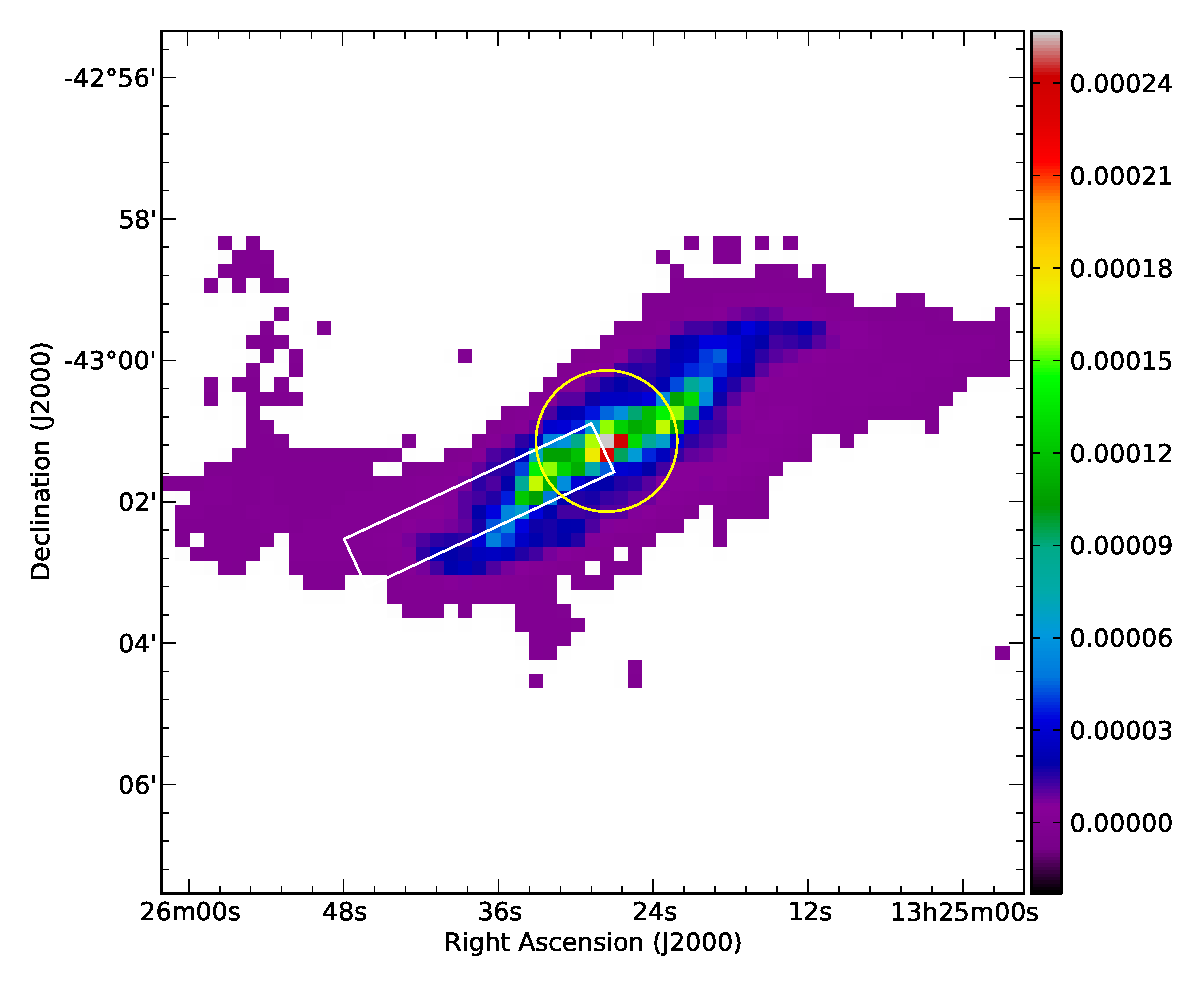
\includegraphics[width=\columnwidth]{CenA_Ftir_image_v1}
\caption{The total infrared flux calculated using Equation~\ref{eqn:Ftir} for Cen~A.  The \emph{Herschel} PACS footprint for our observations is shown as a white rectangle while the yellow circle outlines our SPIRE FTS footprint.  Units are in W~m$^{-2}$~sr$^{-1}$.}
\label{fig:F_tir}
\end{figure}

From Level~0 to Level~1 the PACS spectroscopic observations are processed with the standard pipeline for unchopped scans using the Herschel Interactive Processing Environment \citep[HIPE; ][]{2010ASPC..434..139O} version 9.2 with calibration files FM,41.  For details of the pipeline see \citet{parkin_2013} or the PACS Data Reduction Guide.\footnote{Available for download from the ESA \emph{Herschel} Science Centre. http://herschel.esac.esa.int/hcss-doc-10.0/index.jsp\#pacs\_spec:pacs\_spec}  Level~1 cubes are exported to PACSman v3.5.2 \citep{2012A&A...548A..91L} where each individual spectrum is fit with a second order polynomial and Gaussian function for the baseline and line, respectively.  Lastly, we create a map by projecting the rasters onto a common grid with a pixel scale of 3.133$\arcsec$.  In Figure~\ref{fig:pacs_spec_maps} we show the final mosaicked observations for the [C~\textsc{ii}]$_{158}$, [N~\textsc{ii}]$_{122}$, [O~\textsc{i}]$_{63}$, [O~\textsc{i}]$_{145}$ and [O~\textsc{iii}]$_{88}$ fine structure lines.

%http://herschel.esac.esa.int/hcss-doc-10.0/index.jsp#pacs_spec:pacs_spec
\begin{deluxetable}{lcccccc}
\tabletypesize{\small}
\tablecolumns{7}
\tablecaption{Basic details of the \emph{Herschel} spectroscopic observations of Centaurus~A\label{table: herschel_char}}
\tablewidth{0pt}
\tablehead{
\colhead{Line} & \colhead{Wavelength} & \colhead{OBSID} & \colhead{Date of} & \colhead{Map Size}
 	& \colhead{FWHM\tablenotemark{a}} & \colhead{Integration} \\
                   & \colhead{($\mu$m)}   &            & \colhead{Observation}
    & \colhead{$\arcmin\times\arcmin$} & \colhead{($\arcsec$)} & \colhead{Time (s)}}
 \startdata
 [O\,\textsc{i}]       & 63.184     & 1342223819 & 2011 Jul 9 & 0.72~$\times$~4.0
 	& $\sim$9.3             & 1886 \\
 $[$O\,\textsc{iii}$]$ & 88.356     & 1342223817 & 2011 Jul 9 & 0.72~$\times$~4.0
 	& $\sim$9.3             & 3194 \\
 $[$N\,\textsc{ii}$]$  & 121.898    & 1342223818 & 2011 Jul 9 & 0.72~$\times$~4.0
 	& $\sim$10              & 3198  \\
 $[$O\,\textsc{i}$]$   & 145.525    & 1342223815 & 2011 Jul 9 & 0.72~$\times$~4.0
 	& $\sim$11              & 5840  \\
 $[$C\,\textsc{ii}$]$  & 157.741    & 1342223816 & 2011 Jul 9 & 0.72~$\times$~4.0
 	& $\sim$11.5            & 1886  \\
 $[$N\,\textsc{ii}$]$  & 205.178    & 1342204036 & 2010 Aug 23 & $\sim2\arcmin$~diameter circle
 	& $17$                  & 17843 \\
 \enddata
 \tablenotetext{a}{Values are from the PACS Observer's Manual and the SPIRE Observers' Manual.}
\end{deluxetable}

\subsection{SPIRE spectroscopy}\label{spire_spec}
The SPIRE Fourier Transform Spectrometer observation of Centaurus~A consists of a single pointing with full Nyquist sampling and high spectral resolution.  The 205~$\mu$m line comes from observations using the SPIRE short wavelength (SSW) bolometer array, consisting of 37 hexagonally arranged bolometers with a combined total field-of-view of 2.6$\arcmin$ (although only bolometers within the central $\sim 2.0\arcmin$ are well calibrated).\footnote{Hereafter SPIRE~OM.  Document HERSCHEL-DOC-0798 version 2.4 (June 2011), is available from the ESA \emph{Herschel} Science Centre.}

We processed the observation using HIPE v11.0 developer's build 2652 and calibration set v10.1 using the standard pipeline (see \citet{parkin_2013} for details), then fit the resulting spectral line in each bolometer with a sinc function.  Finally, a map is produced by integrating over each line at a resolution of $\sim 16\arcsec$ and with a 12$\arcsec$ pixel scale.

\subsection{Ancillary Data}
We also incorporate previously published PACS photometry at 70 and 160~$\mu$m \citep{2012MNRAS.422.2291P}.  These data have been reprocessed using HIPE v9.0 (calibration file set FM,41) and \textsc{Scanamorphos} v21 and were set to a final pixel scale of 1.4 and 2.85~$\arcsec$ for the 70 and 160~$\mu$m maps, respectively.  From the same paper we also make use of the CO($J=3-2$) observations taken at the JCMT.  Lastly, we make use of the \emph{Spitzer} MIPS 24~$\mu$m data, reprocessed as described in \citep{2012MNRAS.423..197B}.

\subsection{Final Steps for Analysis}\label{prep_analysis}
The PACS and SPIRE spectroscopy were convolved to a common resolution matching that of our CO($J = 3-2$) observations from the JCMT (14$\arcsec$) using Gaussian kernels.  The MIPS 24~$\mu$m and PACS 70 and 160~$\mu$m maps were convolved to the same resolution using the appropriate kernels from \citet{2011PASP..123.1218A}.  All of our maps were resampled onto a pixel scale of 12$\arcsec$, such that each pixel is mostly independent.  Lastly, we mask out all detections below 5$\sigma$ in our spetroscopic maps to ensure robust line ratios.

Calibration uncertainties are 4\% for the MIPS 24~$\mu$m photometry\footnote{MIPS Instrument Handbook, available at http://irsa.ipac.caltech.edu/data/SPITZER/docs/mips/\-mipsinstrumenthandbook/home/}, 5\% for the PACS 70 and 160~$\mu$m maps (PACS~OM).  The PACS spectroscopic maps have 30\% calibration uncertainties (PACS~OM) while the SPIRE FTS map has a 7\% calibration uncertainty (SPIRE~OM).

%%%%%%%%%%%%%%%%%%%%%%%%%%%%%%%%%%%%%%%%%%%%%%%%%%%%
\section{Results}\label{results}

\subsection{Morphological Properties}\label{properties}
Figure~\ref{fig:pacs_spec_maps} shows our PACS and SPIRE spectroscopic maps at their native resolution and pixel scale.  The [C~\textsc{ii}] emission, tracing both neutral and ionized gas, shows a smooth decrease overall from near the center of the galaxy to the edge of our map.  There is a curve in the strongest [C~\textsc{ii}] emission, which is coincident with the 70~$\mu$m emission shown in contours.  The peak is at the end of this bend, and is a factor of roughly 100 times higher than the outer part of the map.  This peak has also been seen previously in the \emph{Herschel} PACS 160~$\mu$m band as well as the three SPIRE photometric bands at 250, 350 and 500~$\mu$m and in CO($J=3-2$) emission \citep{2012MNRAS.422.2291P}.  Furthermore, \citet{2006ApJ...645.1092Q} presented \emph{Spitzer} Infrared Array Camera (IRAC) photometry that demonstrate a parallelogram shaped ring, coincident with our [C~\textsc{ii}] observations.  The total flux in our [C~\textsc{ii}] map is $(4.268 \pm 0.002 (\mathrm{stat}) \pm 1.280 (\mathrm{cal})) \times 10^{-14}$~W~m$^{-2}$, over an area of approximately 11200~square arcseconds.  Our value is in fairly good agreement with \citet{2000A&A...355..885U}, who found a total flux for their center and south-east pointings (those which overlap our observations) of $3.83 \times 10^{-14}$~W~m$^{-2}$ covering a total area of 11100~square arcseconds given ISO's 70$\arcsec$ beam.  Any disagreement likely is due to the fact that our observations are not entirely coincident with theirs.

The [O~\textsc{i}]$_{63}$ and [O~\textsc{i}]$_{145}$ maps reveal the distribution of neutral gas, and they too show a curve downward in emission, as seen in the [C~\textsc{ii}] emission, with the intensity falling off radially away from the center region.  The total flux in these lines is $(1.171 \pm 0.002 (\mathrm{stat}) \pm 0.351 (\mathrm{cal})) \times 10^{-14}$~W~m$^{-2}$ and $(1.006 \pm 0.003 (\mathrm{stat}) \pm 0.302 (\mathrm{cal})) \times 10^{-15}$~W~m$^{-2}$ at 63 and 145~$\mu$m, respectively.  Interestingly, the strongest emission peaks in the innermost region, unlike the [C~\textsc{ii}] emission, which shows a weaker enhancement at the center compared to the the tip of the curve.  Peaked central emission in [O~\textsc{i}]$_{63}$ has also been observed by \citet{parkin_2013} in the nucleus of M51, where it was attributed to shocks produced by the Seyfert~2 nucleus.  Cen~A has a strong central active galactic nucleus (AGN), thus it is possible we see the same type of behaviour in the center as in M51.  This is further supported by the fact that while our [O~\textsc{i}]$_{145}$ flux is in good agreement with \citet{2000A&A...355..885U}, who found a total flux of approximately $1.1 \times 10^{-15}$~W~m$^{-2}$ in their center pointing with ISO, their [O~\textsc{i}]$_{63}$ flux is $1.96 \times 10^{-14}$~W~m$^{-2}$ in the center alone, with another $5.1 \times 10^{-15}$~W~m$^{-2}$ in their south-eastern pointing.  Thus, a large fraction of the total [O~\textsc{i}]$_{63}$ flux likely originates in the nucleus, outside the range of our observations.

\begin{figure*}
 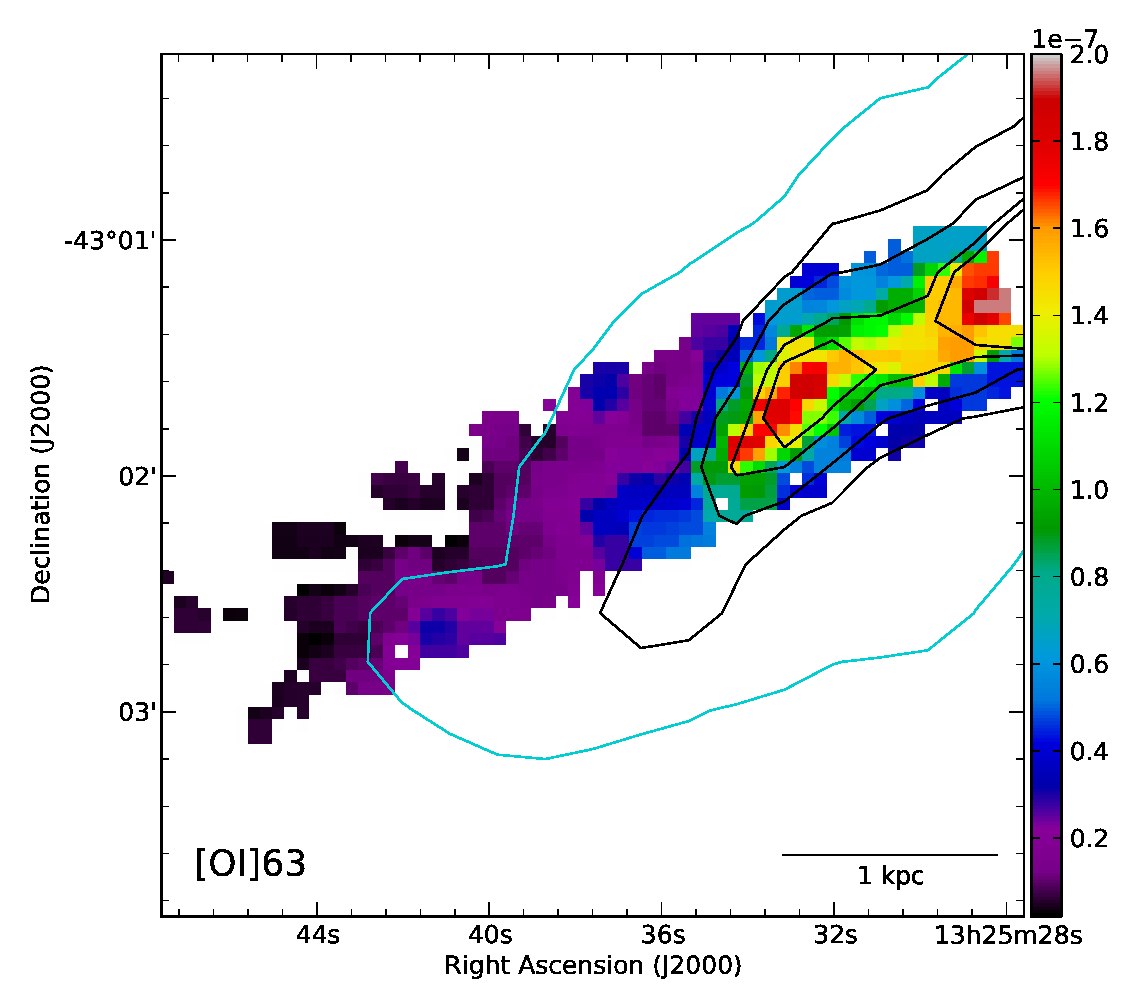
\includegraphics[width=7.2cm]{CenA_OI63_unconvolved_image_v1_cropped}
 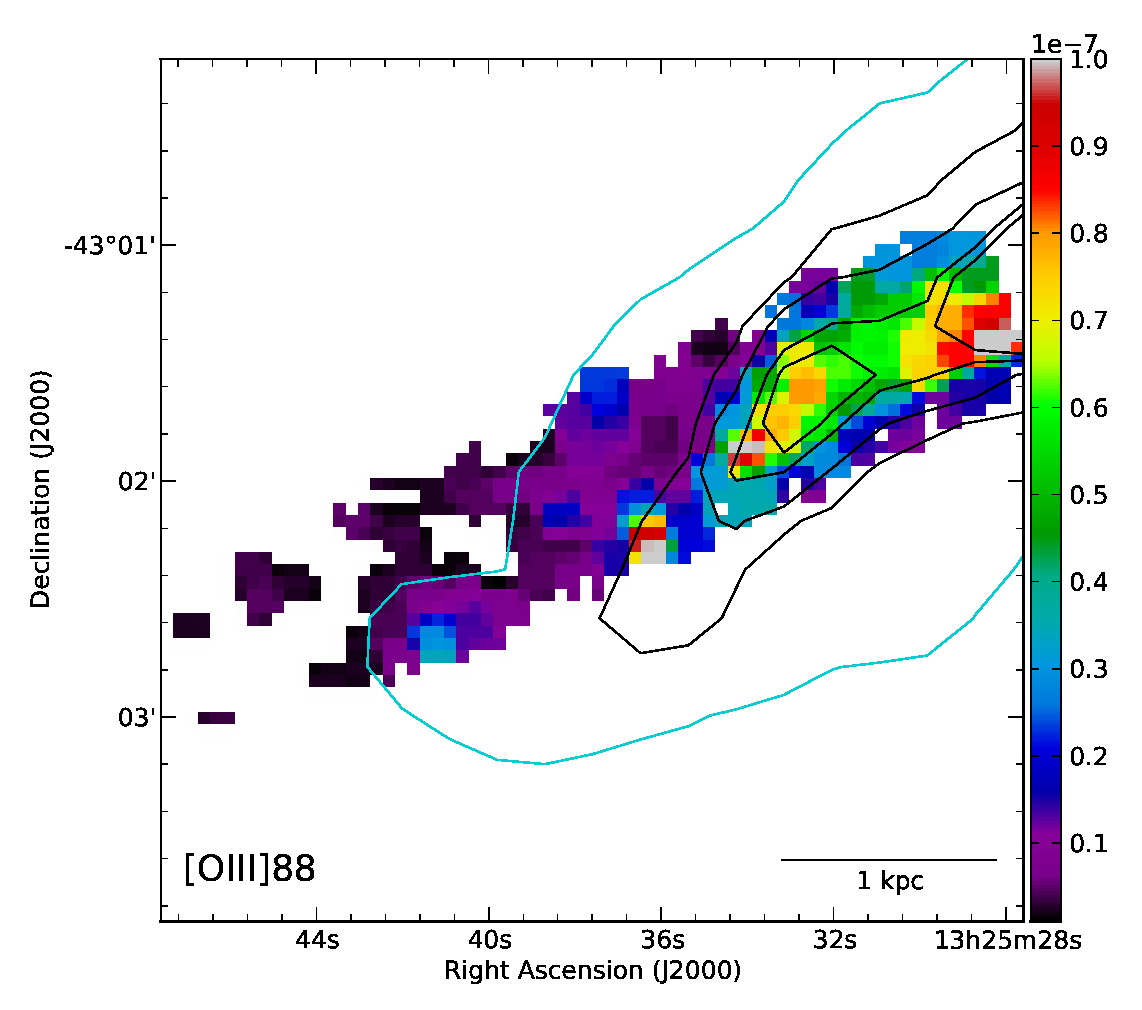
\includegraphics[width=7.2cm]{CenA_OIII88_unconvolved_image_v1_cropped}
 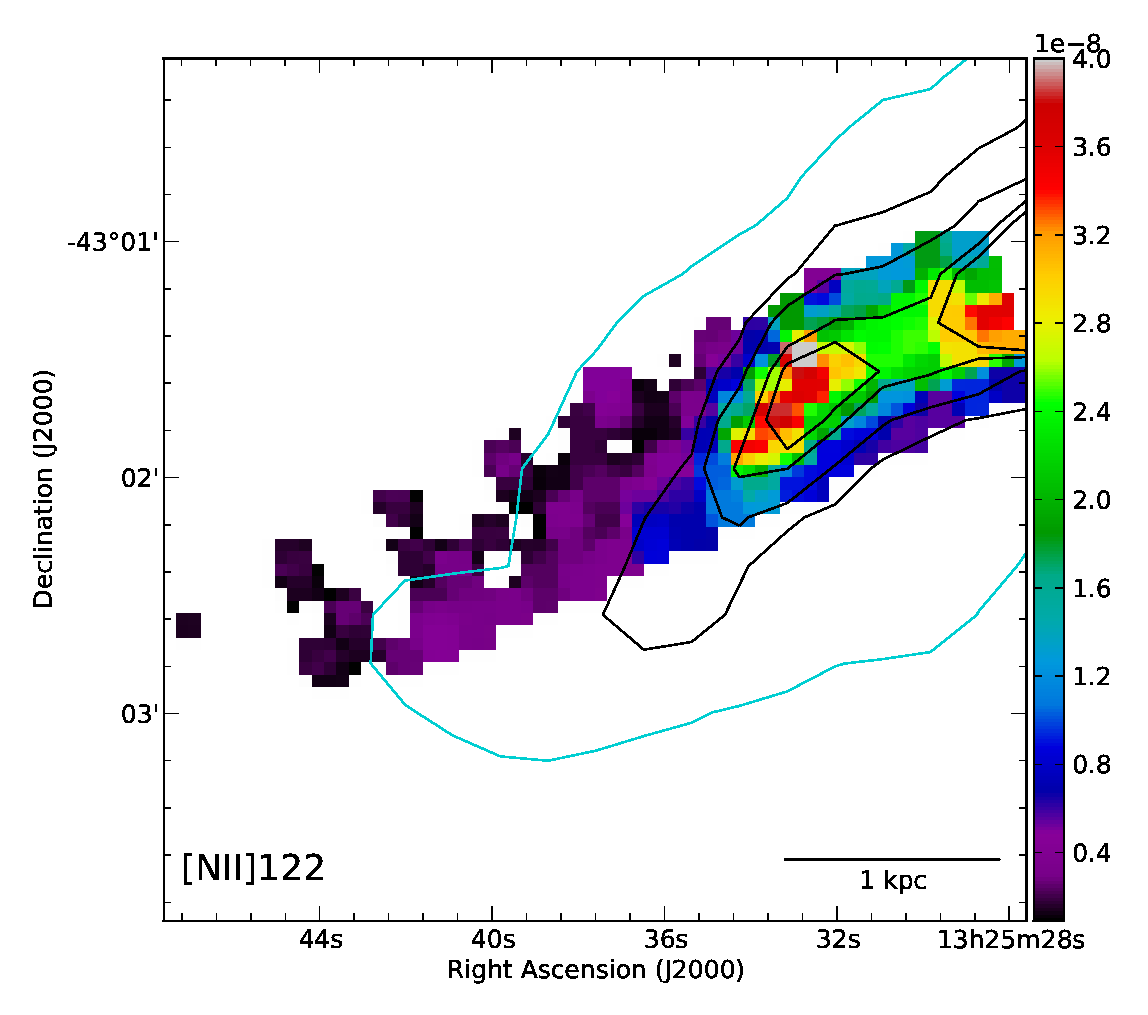
\includegraphics[width=7.2cm]{CenA_NII122_unconvolved_image_v1_cropped}
 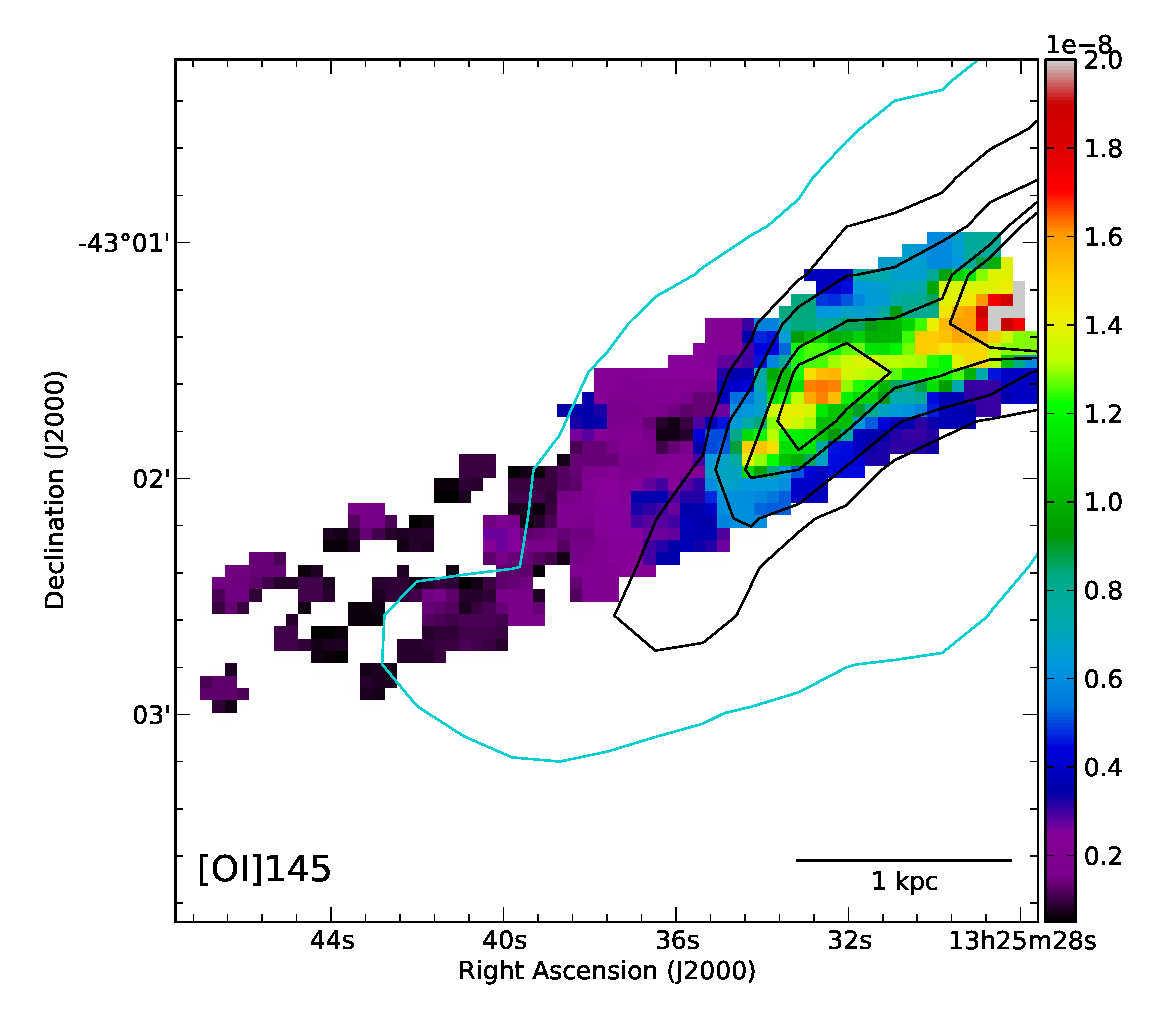
\includegraphics[width=7.2cm]{CenA_OI145_unconvolved_image_v1_cropped}
 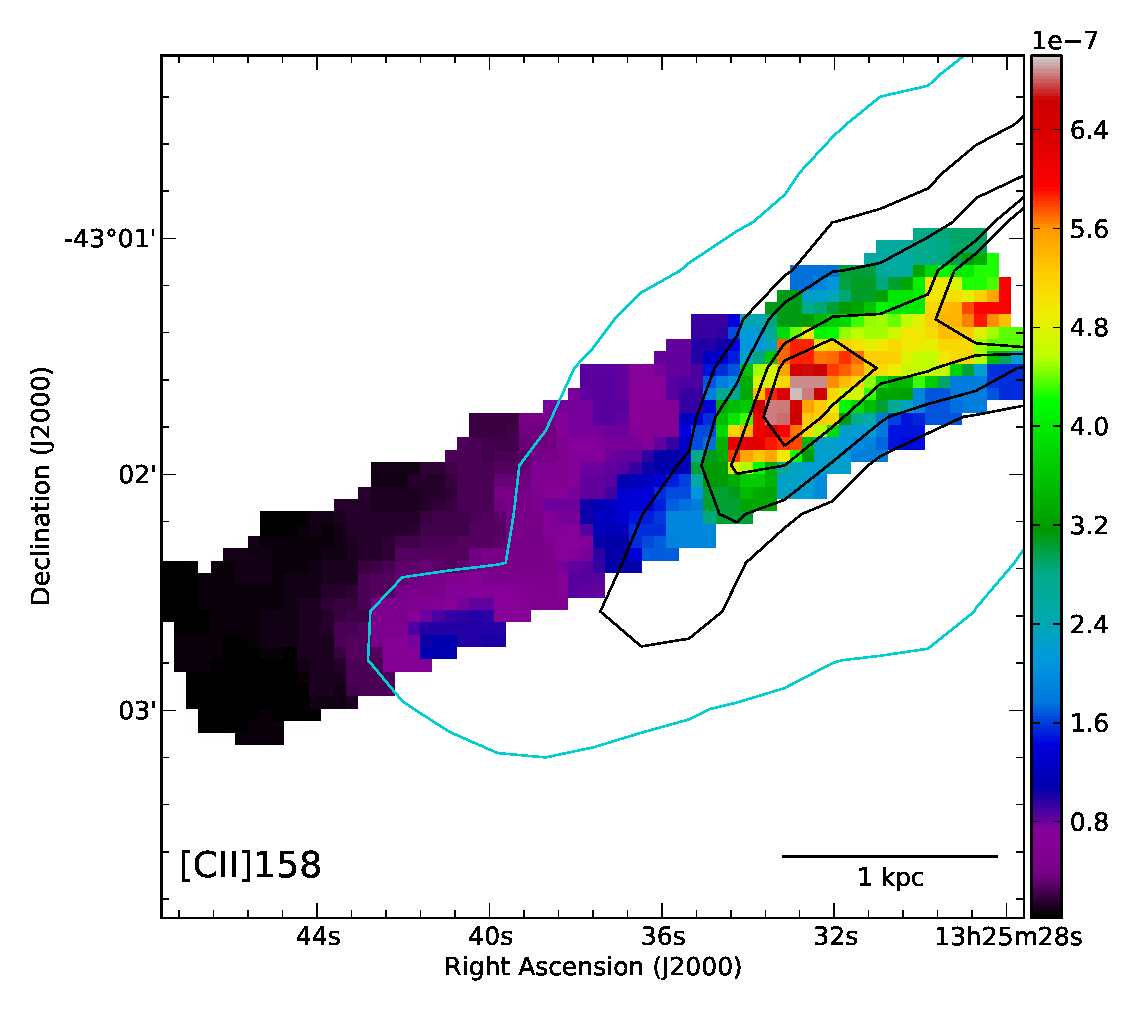
\includegraphics[width=7.2cm]{CenA_CII157_unconvolved_image_v1_cropped}
 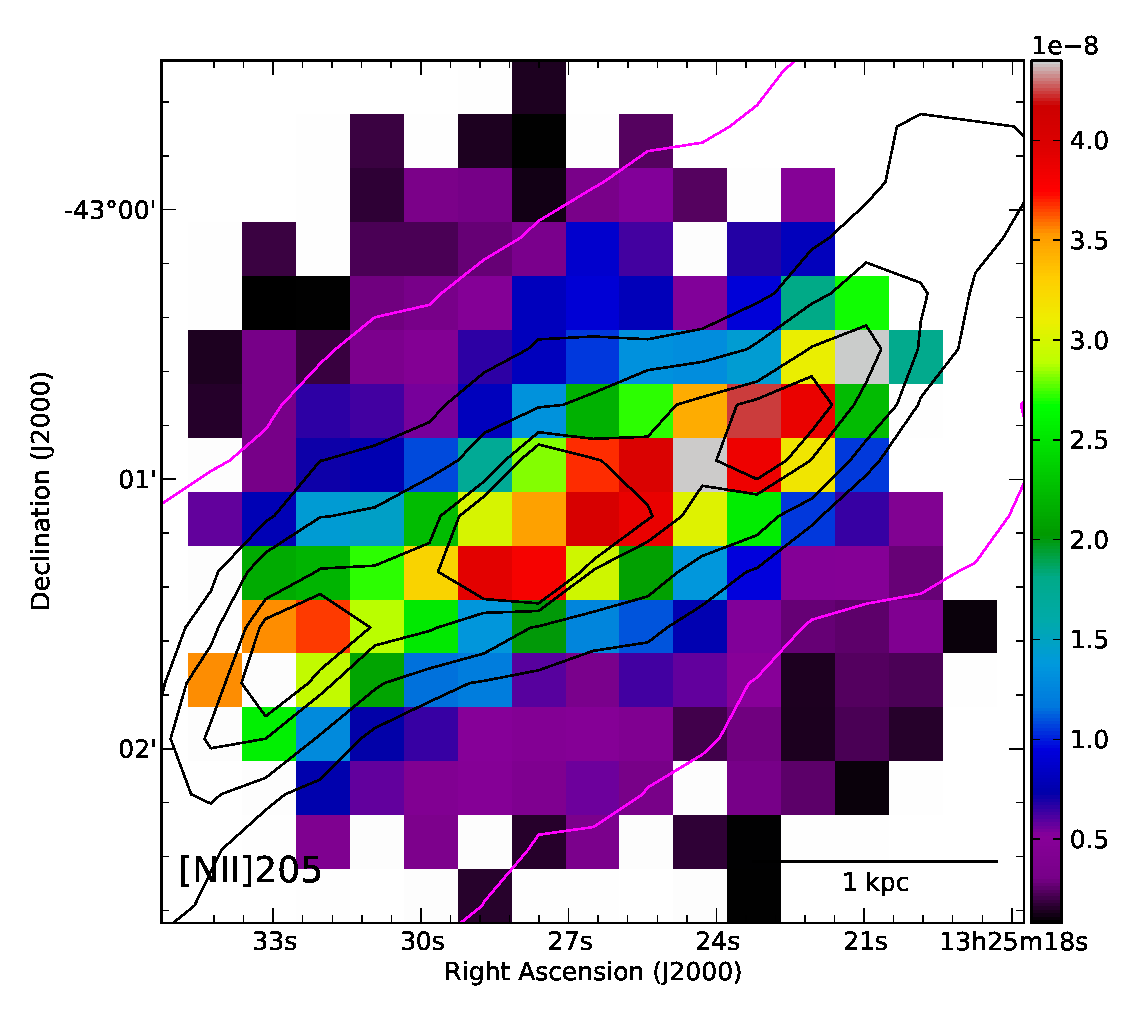
\includegraphics[width=7.2cm]{CenA_NII205_unconvolved_image_v1}
\caption{The maps of our \emph{Herschel} PACS and SPIRE spectroscopic observations of the far-infrared cooling lines at their native resolution and pixel scale.  We have applied a 3$\sigma$ cut to these maps to highlight robust detections.  Units in all images are W~m$^{-2}$~sr$^{-1}$.  Contours from the \emph{Herschel} PACS 70~$\mu$m photometric map are overlaid on top with the levels corresponding to $3 \times 10^{-6}$,  $1.5 \times 10^{-5}$,$3.0 \times 10^{-5}$,$6.0 \times 10^{-5}$ and $7.5 \times 10^{-5}$~W~m$^{-2}$~sr$^{-1}$.}
\label{fig:pacs_spec_maps}
\end{figure*}

\begin{deluxetable}{lcc}
\tabletypesize{\small}
\tablecolumns{3}
\tablecaption{Total integrated flux for the PACS cooling lines in Cen~A.\label{tbl:int_flux}}
\tablewidth{0pt}
\tablehead{
\colhead{Line} & \colhead{$F$ ($10^{-14}$~W~m$^{-2}$)\tablenotemark{a}}
					& \colhead{Area\tablenotemark{b} ($\sq\arcsec$)}}
  \startdata
 $[$C\,\textsc{ii}]         & $4.268 \pm 0.002$ & 11232 \\
 $[$N\,\textsc{ii}]$_{122}$ & $0.2014 \pm 0.0004$ & 9792  \\
 $[$O\,\textsc{i}]$_{63}$   & $1.171 \pm 0.002$ & 11080 \\
 $[$O\,\textsc{i}]$_{145}$  & $0.1006 \pm 0.0003$ & 10512 \\
 $[$O\,\textsc{iii}]        & $0.550 \pm 0.001$ & 10656 \\
 $[$N\,\textsc{ii}]$_{205}$ & $0.642 \pm 0.007$ & 22752 \\
 \enddata
 \tablenotetext{a}{Total integrated flux of each atomic fine structure line we observed for Cen~A.  Note that the uncertainties exclude those due to calibrations.}
 \tablenotetext{b}{The area in square arcseconds over which each total is calculated.  The variations reflect the number of good pixels included in the sum.}
\end{deluxetable}

The [N~\textsc{ii}]$_{122}$, [N~\textsc{ii}]$_{205}$ and [O~\textsc{iii}] fine structure lines trace ionized gas.  The ionized gas shown by the [N~\textsc{ii}]$_{122}$ and [O~\textsc{iii}] line emission traces the neutral gas and dust emission well in the inner half of the map with sparse detections at greater than a 3$\sigma$ level further out.  While there is an enhancement near the center of the galaxy, the peak of the ionized gas as traced by the [N~\textsc{ii}]$_{122}$ emission is at the tip of the curve and is a factor of 2 times greater than the other parts of the inner curve, and an order of magnitude larger than the outer parts of the map.  In contrast, the peak emission in [O~\textsc{iii}] is coincident with the peak of the [O~\textsc{i}]$_{63}$ and [O~\textsc{i}]$_{145}$.  There are also a few other peaks of emission, one at the tip of the curve and a little pocket in the middle of the strip in the south, which is weakly visible in the [N~\textsc{ii}]$_{122}$, but not in the maps of neutral gas.  The total flux of [O~\textsc{iii}] in our observations is $(5.50 \pm 0.01 (\mathrm{stat}) \pm 1.65 (\mathrm{cal})) \times 10^{-15}$~W~m$^{-2}$, while the total flux in the [N~\textsc{ii}]$_{122}$ line is $2.014 \pm 0.004 (\mathrm{stat}) \pm 0.604 (\mathrm{cal})) \times 10^{-15}$~W~m$^{-2}$.  \citet{2000A&A...355..885U} find a flux of $7.2 \times 10^{-15}$~W~m$^{-2}$ in [O~\textsc{iii}] for the center pointing, and $1.5 \times 10^{-15}$~W~m$^{-2}$ in [N~\textsc{ii}]$_{122}$ for their center pointing, and an upper limit in their south-east pointing of the same flux.

The area covered by our [N~\textsc{ii}]$_{205}$ map is different than the other five lines we present here, as the observations are centered on the nucleus of the galaxy.  We see that there is a strong detection across the disk, with an emission peak that is roughly a factor of 40 larger than emission detected above and below the plane.  A comparison between the 70~$\mu$m contours and the [N~\textsc{ii}]$_{205}$ shows that the peak slightly to the northwest of the center is also detected in the ionized gas, and that the warp in the disk is also visible in the [N~\textsc{ii}]$_{205}$ line.  The total flux in this map is $(6.42 \pm 0.07 (\mathrm{stat}) \pm 0.45 (\mathrm{cal})) \times 10^{-15}$~W~m$^{-2}$.

Lastly, in Figure~\ref{fig:F_tir} we show the total infrared flux of Cen~A, which is needed for our comparison of observations with the PDR model in Section~\ref{pdr_model}.  We calculated the total infrared flux using \emph{Spitzer} MIPS 24~$\mu$m photometry \citep{2012MNRAS.423..197B}, PACS 70 and 160~$\mu$m photometry \citep{2012MNRAS.422.2291P}, and the empirically determined equation for the total infrared flux (or luminosity) from \citet{2013MNRAS.431.1956G},

\begin{eqnarray}\label{eqn:Ftir}
F_{\mathrm{TIR}} = (2.133 \pm 0.095)\nu_{24} F_{24} + (0.681 \pm 0.028)\nu_{70} F_{70}
	\nonumber \\
	+ (1.125 \pm 0.010) \nu_{160} F_{160}.
\end{eqnarray}

This map covers the entire disk of Cen~A; however, we only use the region overlapping with our spectroscopic maps for our analysis.

\subsection{Line Ratio Diagnostics}\label{subsec:ratio}
\subsubsection{[C~\textsc{ii}], [O~\textsc{i}]$_{63}$ and $F_{\mathrm{TIR}}$}
The [C~\textsc{ii}]/$F_{\mathrm{TIR}}$ line ratio for Cen~A is shown in the top left panel of Figure~\ref{fig:cena_ratios}.  At first glance there does not appear to be any trend with radius; however, when compared with the 70~$\mu$m continuum emission overlaid in contours, it appears there is a slight increase with radius ranging from approximately $3 \times 10^{-3}$ in the center, to $6 \times 10^{-3}$ in the middle of the strip, and then a decrease in the outermost region of the map, indicating a slight deficit toward the center of the galaxy.  The average of this ratio across our strip is $\sim (5 \pm 1) \times 10^{-3}$.  This ratio is often given by  [C~\textsc{ii}]/$F_{\mathrm{FIR}}$, where $F_{\mathrm{FIR}} = F_{\mathrm{TIR}}/1.3$ \citep{2008A&A...479..703G} is the far-infrared flux.  Correspondingly, our observations correspond to a range of $3.9 \times 10^{-3}$ to $7.8 \times 10^{-3}$ and an average of $(6.5 \pm 1.3)\times 10^{-3}$ for the [C~\textsc{ii}]/$F_{\mathrm{FIR}}$ line ratio.

This ratio has been probed on resolved scales in other galaxies, including M82 \citep[10$^{-3}-10^{-2}$; ][]{2013A&A...549A.118C}, NGC~6946 and NGC~1313 \citep[$8\times 10^{-3}$; ][]{2002AJ....124..751C}, M51 \citep[$4 \times 10^{-3}$; ][]{parkin_2013} and the Orion Molecular Cloud in the Galaxy \citep[$3 \times 10^{-3}$; ][]{1993ApJ...404..219S}.  Our observed line ratio for Cen~A is in good agreement with the values in other galaxies as well as a previous determination of this line ratio by \citet{2001A&A...375..566N} of $3.2 \times 10^{-3}$.  On global scales, the [C~\textsc{ii}] deficit appears when comparing ULIRGs to normal galaxies.  For example, \citet{1998ApJ...504L..11L} and \citet{2003ApJ...594..758L} find ULIRGs have a [C~\textsc{ii}]/$F_{\mathrm{FIR}}$ line ratio of less than $5 \times 10^{-4}$, which is an order of magnitude lower than in normal galaxies \citep{1985ApJ...291..755C, 2001ApJ...561..766M, 2001A&A...375..566N}.  Thus, we believe that the deficit observed in Cen~A is not of the same degree as in ULIRGs, but is similar to that found in M51 \citep{parkin_2013}.

\begin{figure*}
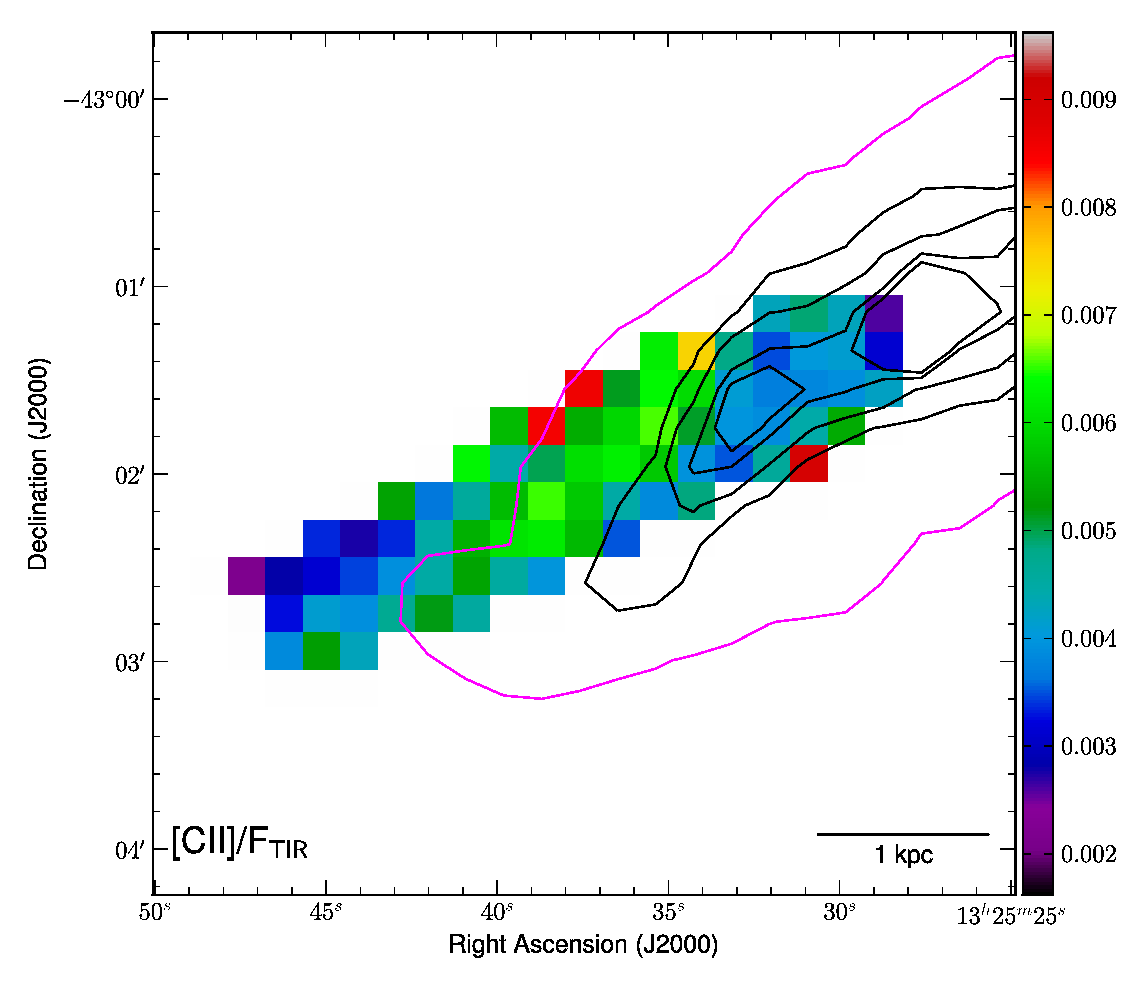
\includegraphics[width=\columnwidth]{CenA_CIIonFtir_image_v1}
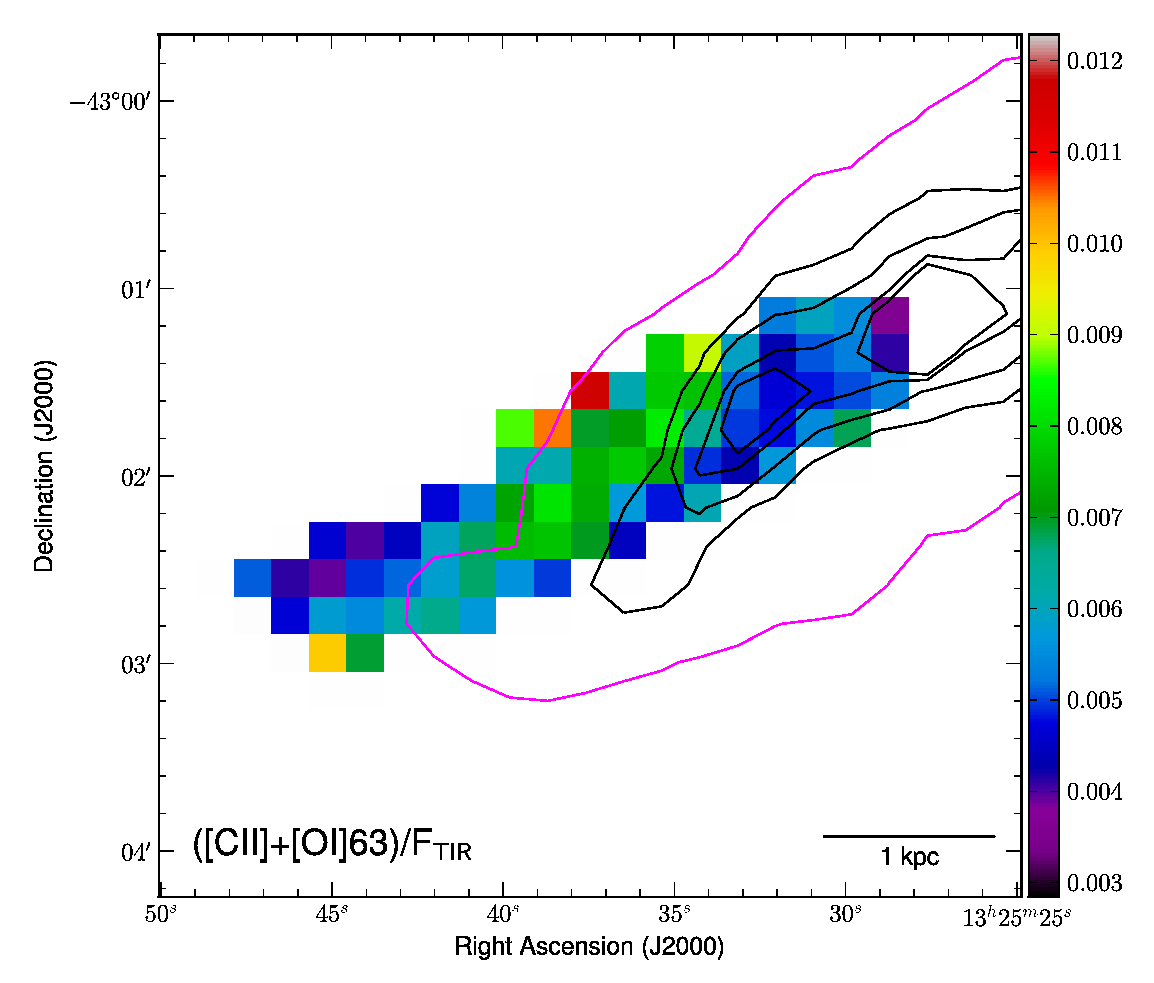
\includegraphics[width=\columnwidth]{CenA_CIIOI63onFtir_image_v1}
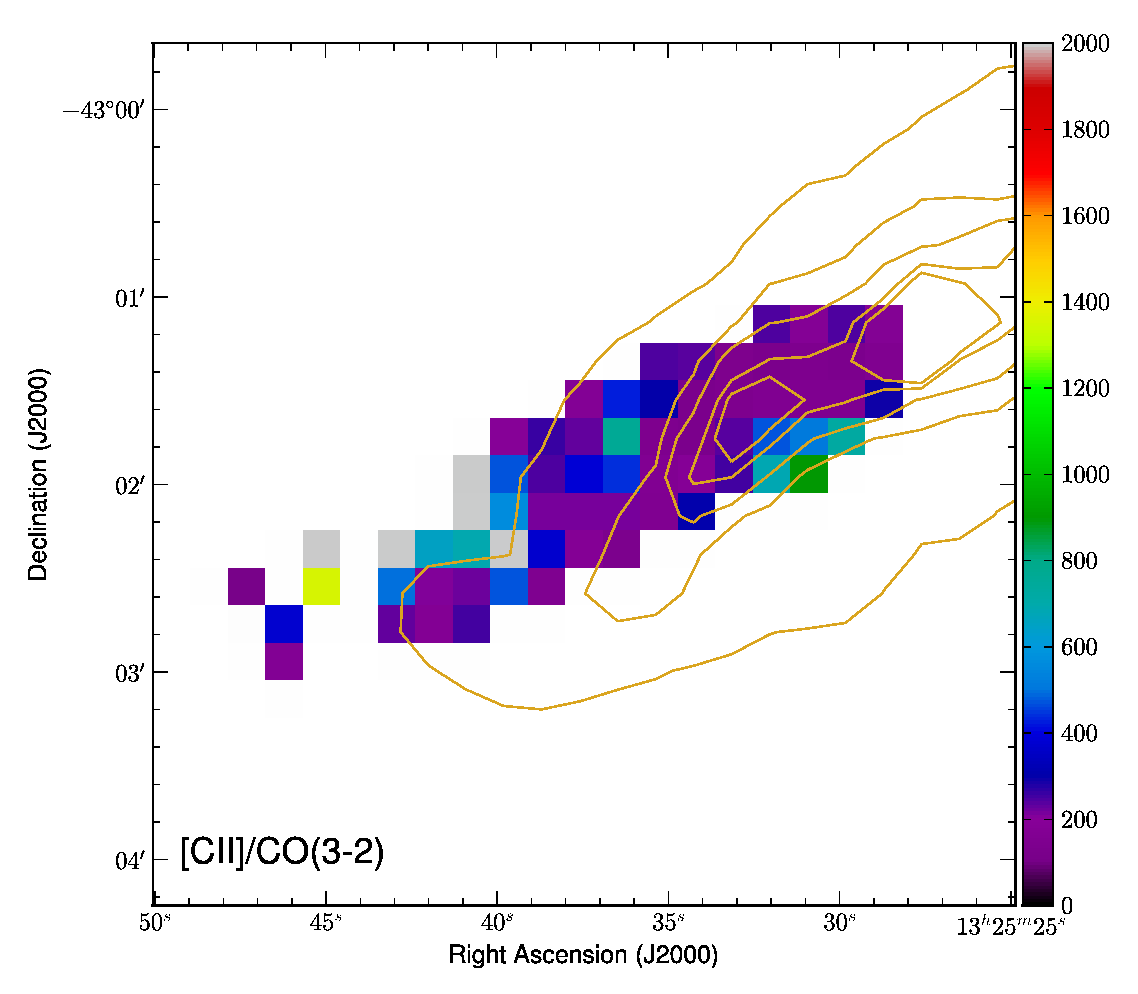
\includegraphics[width=\columnwidth]{CenA_CIIonCO3-2_image}
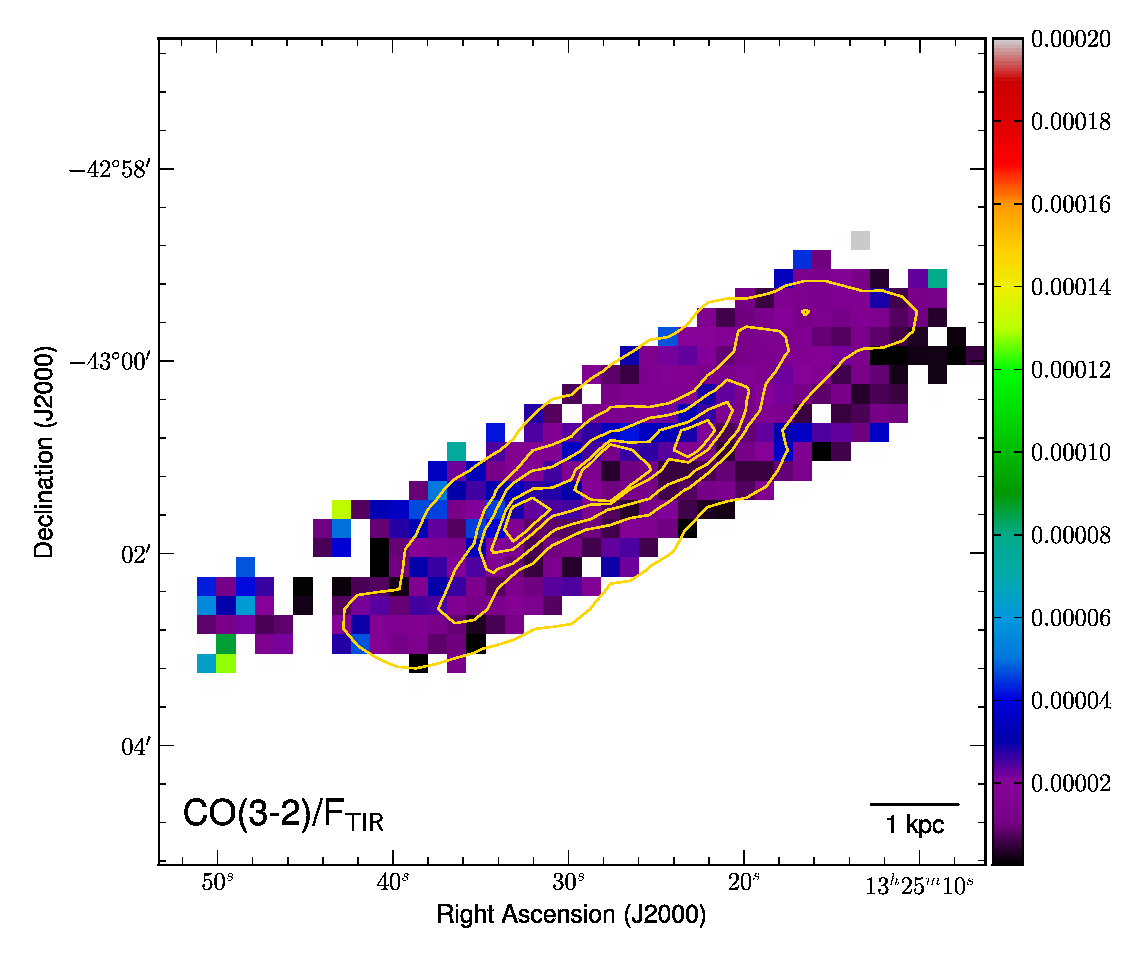
\includegraphics[width=\columnwidth]{CenA_CO3-2onFtir_image_v1}
\caption{Maps of the [C~\textsc{ii}]/$F_{\mathrm{TIR}}$ (\emph{top left}), ([C~\textsc{ii}]+[O~\textsc{i}]$_{63}$)/$F_{\mathrm{TIR}}$ (\emph{top right}), [C~\textsc{ii}]/CO($J=3-2$) (\emph{bottom left}), and CO($J=3-2$)/$F_{\mathrm{TIR}}$ (\emph{bottom right}) line ratios for our observed region of Cen~A.  Contours of the \emph{Herschel} PACS 70~$\mu$m emission are overlaid on top, with the same contour levels as in Figure~\ref{fig:pacs_spec_maps}.}
\label{fig:cena_ratios}
\end{figure*}

The line ratio of ([C~\textsc{ii}]+[O~\textsc{i}]$_{63}$)/$F_{\mathrm{TIR}}$ (top right panel of Figure~\ref{fig:cena_ratios}) gives us an indication of the heating efficiency in Cen~A.  The [C~\textsc{ii}] and [O~\textsc{i}]$_{63}$ lines are the dominant coolants in the neutral gas of PDRs.  Thus, their strength tells us how many FUV photons contribute to gas heating, assuming every free electron produced via the photoelectric effect eventually results in the emission of a [C~\textsc{ii}] or [O~\textsc{i}]$_{63}$ photon.  This value is then divided by the total infrared flux, which indicates how many FUV photons result in dust heating if we assume all dust grains irradiated by FUV flux eventually re-emit infrared continuum emission.  Like the [C~\textsc{ii}]/$F_{\mathrm{TIR}}$ line ratio, the heating efficiency shows a slight increase with radius, with values ranging from $4 \times 10^{-3}$ to $8 \times 10^{-3}$ with an average of $(6 \pm 2) \times 10^{-3}$.  This suggests the heating efficiency is lower toward the center of the galaxy where there is a harder FUV flux as indicated by the [O~\textsc{iii}] emission, which also peaks in the center.  Our value for this ratio is consistent with previous measurements in Cen~A. \citet{2000A&A...355..885U} find a value of $6 \times 10^{-3}$ in their center and south-east regions, but their 70$\arcsec$ resolution could not identify the radial trend that we see here.  In other galaxies this ratio typically varies between $1.6 \times 10^{-3}$ and 10$^{-2}$, such as is found by \citet{2001ApJ...561..766M}, who studied 60 normal, star forming galaxies on global scales.

We can also look at the heating efficiency as a function of infrared color, 70$\mu$m/160$\mu$m (which indicates dust temperature), as shown in the top panel of Figure~\ref{fig:heat_eff}.  Here we have divided our strip into eight radial bins as shown by the schematic in Figure~\ref{fig:pdr_plots} (top left panel), and each point represents the average value in each bin with the standard deviation.  The innermost bin (shown in red) has value of $\sim 5 \times 10^{-3}$, then we see an increase in the middle bins of up to almost $8 \times 10^{-3}$ (shown in blue), then a decrease again in the outermost bins.  This trend is emphasized in the bottom panel of Figure~\ref{fig:heat_eff}, where we show a plot of the heating efficiency as a function of dust temperature, which was determined by \citet{2012MNRAS.422.2291P}.  The innermost bins show the warmest dust.  A decrease in heating efficiency with increasing infrared color (and thus dust temperature) has been previously observed within individual galaxies by \citet{2012A&A...548A..91L} in an H~\textsc{ii} region within the Large Magellanic Cloud, by \citet{2012ApJ...747...81C} in NGC~1097 and NGC~4559, and by \citet{parkin_2013} in M51.

\begin{figure}
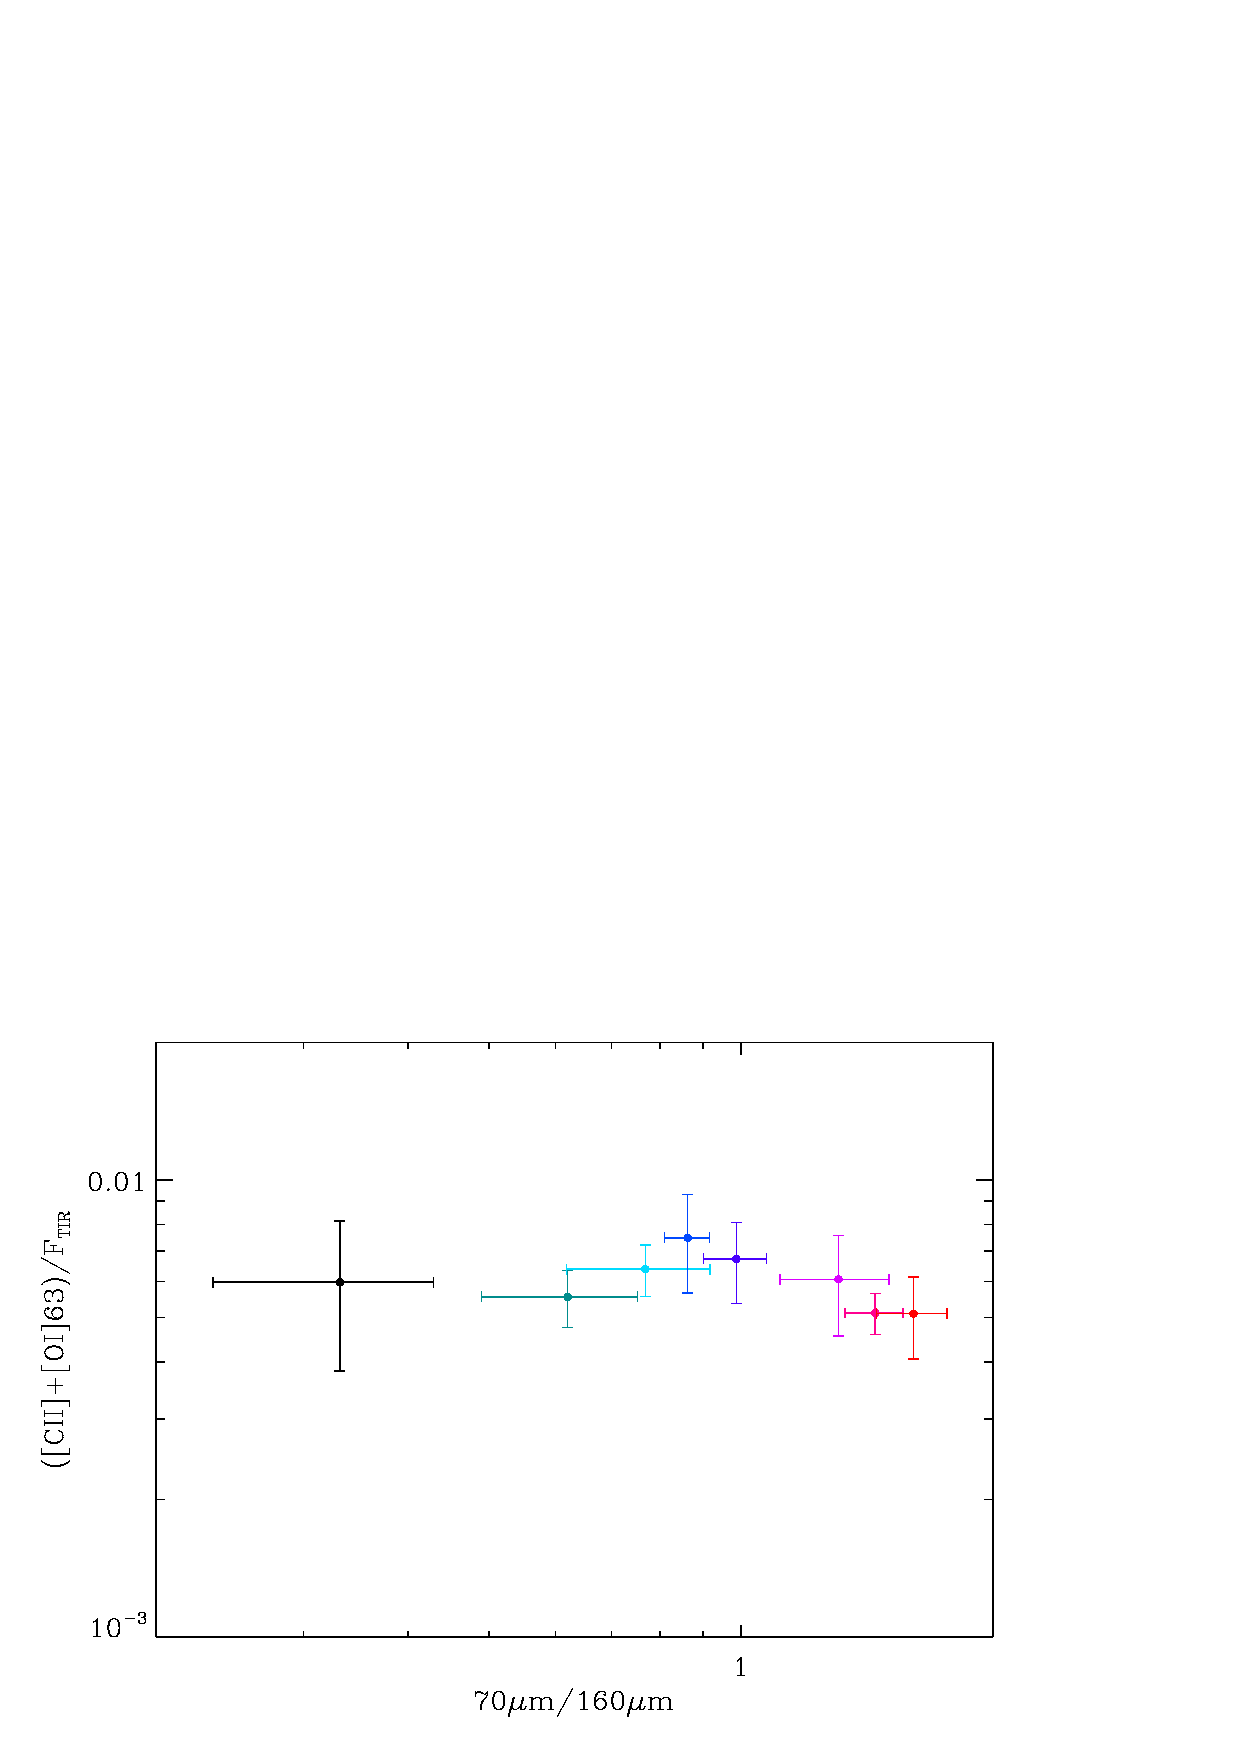
\includegraphics[width=\columnwidth]{CenA_CIIOI63onFtir_vs_70on160_uncorrected_plot_v1}
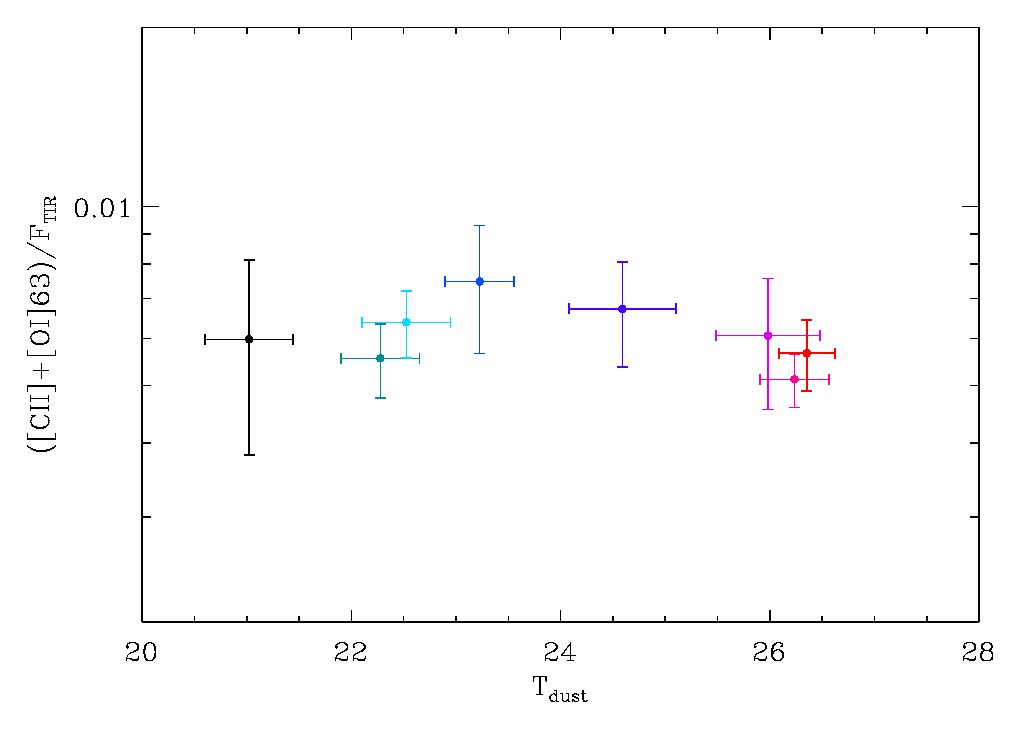
\includegraphics[width=\columnwidth]{CenA_CIIOI63onFtir_vs_Tdust_uncorrected_plot_v1}
\caption{The sum of the [C~\textsc{ii}] and [O~\textsc{i}]$_{63}$ cooling lines divided by the total infrared flux, $F_{\mathrm{TIR}}$ for Cen~A.  Each data point represents the average value within a bin, as described below in Section~\ref{pdr_model}.  Systematic uncertainties due to calibration are not shown.}
\label{fig:heat_eff}
\end{figure}

\subsubsection{Molecular Gas Cooling}
CO can also play a role in the cooling budget, as it too contributes to the cooling via its rotational lines.  In the bottom panel of Figure~\ref{fig:cena_ratios} we show the line ratio CO($J=3-2$)/$F_{\mathrm{TIR}}$ for Cen~A.  This ratio is quite weak, varying from roughly $6.6 \times 10^{-7}$ to $4.6 \times 10^{-5}$, with an average of $(2 \pm 1) \times 10^{-5}$.  There does not appear to be any trend with increasing radius in this line ratio, unlike the other line ratios discussed here.  Assuming the CO($J=3-2$)/CO($J=1-0$) ratio is 0.3, typical for the diffuse ISM\footnote{Note this ratio is calculated when the CO integrated intensities are both in units of K~km~s$^{-1}$.  It becomes 8 when the CO fluxes have been converted to units of W~m$^{-2}$.} \citep{2009ApJ...693.1736W}, these ratios correspond to a CO($J=1-0$)/$F_{\mathrm{TIR}}$ ratio of approximately $8.3 \times 10^{-8}$ to $5.8 \times 10^{-6}$.  The average value of the [C~\textsc{ii}]/CO($J=1-0$) line ratio is $(2.1 \pm 1.3) \times 10^{3}$ across our strip, which is lower than that found for a sample of starburst galaxies and Galactic star forming regions including Cen~A, which is 6300 \citep{1991ApJ...373..423S}.  One possible region for such a discrepancy is that the correlation found in \citet{1991ApJ...373..423S} is for Galactic star forming regions and global values averaged over entire galaxies.  Our observations fall in between these two scales, and perhaps there is more CO emission on the scale of our strip compared to the [C~\textsc{ii}] emission.

By converting the CO flux to a molecular hydrogen mass we can to compare our various line/$F_{\mathrm{TIR}}$ ratios with recent results from \citet{2011ApJ...728L...7G}.  These authors investigated the parameter space of line/$F_{\mathrm{TIR}}$ vs. $L_{\mathrm{TIR}}$/$M_{\mathrm{H}2}$ for a subset of the SHINING sample of galaxies.  The ratio $L_{\mathrm{TIR}}$/$M_{\mathrm{H}2}$ loosely represents the number of stars formed per unit mass of molecular gas per unit of time.  To convert our CO($J=3-2$) integrated intensity to an H$_{2}$ mass, we assume a X$_{\mathrm{CO}}$ factor of $(2 \pm 1) \times 10^{20}$~cm$^{-2}$~(K~km~s$^{-1}$)$^{-1}$, typical for the Milky Way \citep{1988A&A...207....1S}, and a CO($J=3-2$)/CO($J=1-0$) ratio of 0.3, appropriate for the average ISM \citep{2009ApJ...693.1736W}.  Since we do not have global measurements for the various fine structure lines, we opt to instead measure $L_{\mathrm{TIR}}$/$M_{\mathrm{H}2}$ for each of the radial bins (see below) and probe local scales.  In Figure~\ref{fig:sfr} we plot the line/$F_{\mathrm{TIR}}$ ratios vs. the $L_{\mathrm{TIR}}$/$M_{\mathrm{H}2}$ for each of the bins in Cen~A.  Our results are consistent with those from \citet{2011ApJ...728L...7G} at the low end of the $L_{\mathrm{TIR}}$/$M_{\mathrm{H}2}$ scale.  However, we do not probe to high enough scales to see the deficit take effect at $L_{\mathrm{TIR}}$/$M_{\mathrm{H}2} \gtrsim 80$~L$_{\odot}$~M$_{\odot}$ as shown by \citet{2011ApJ...728L...7G}. 

\begin{figure}
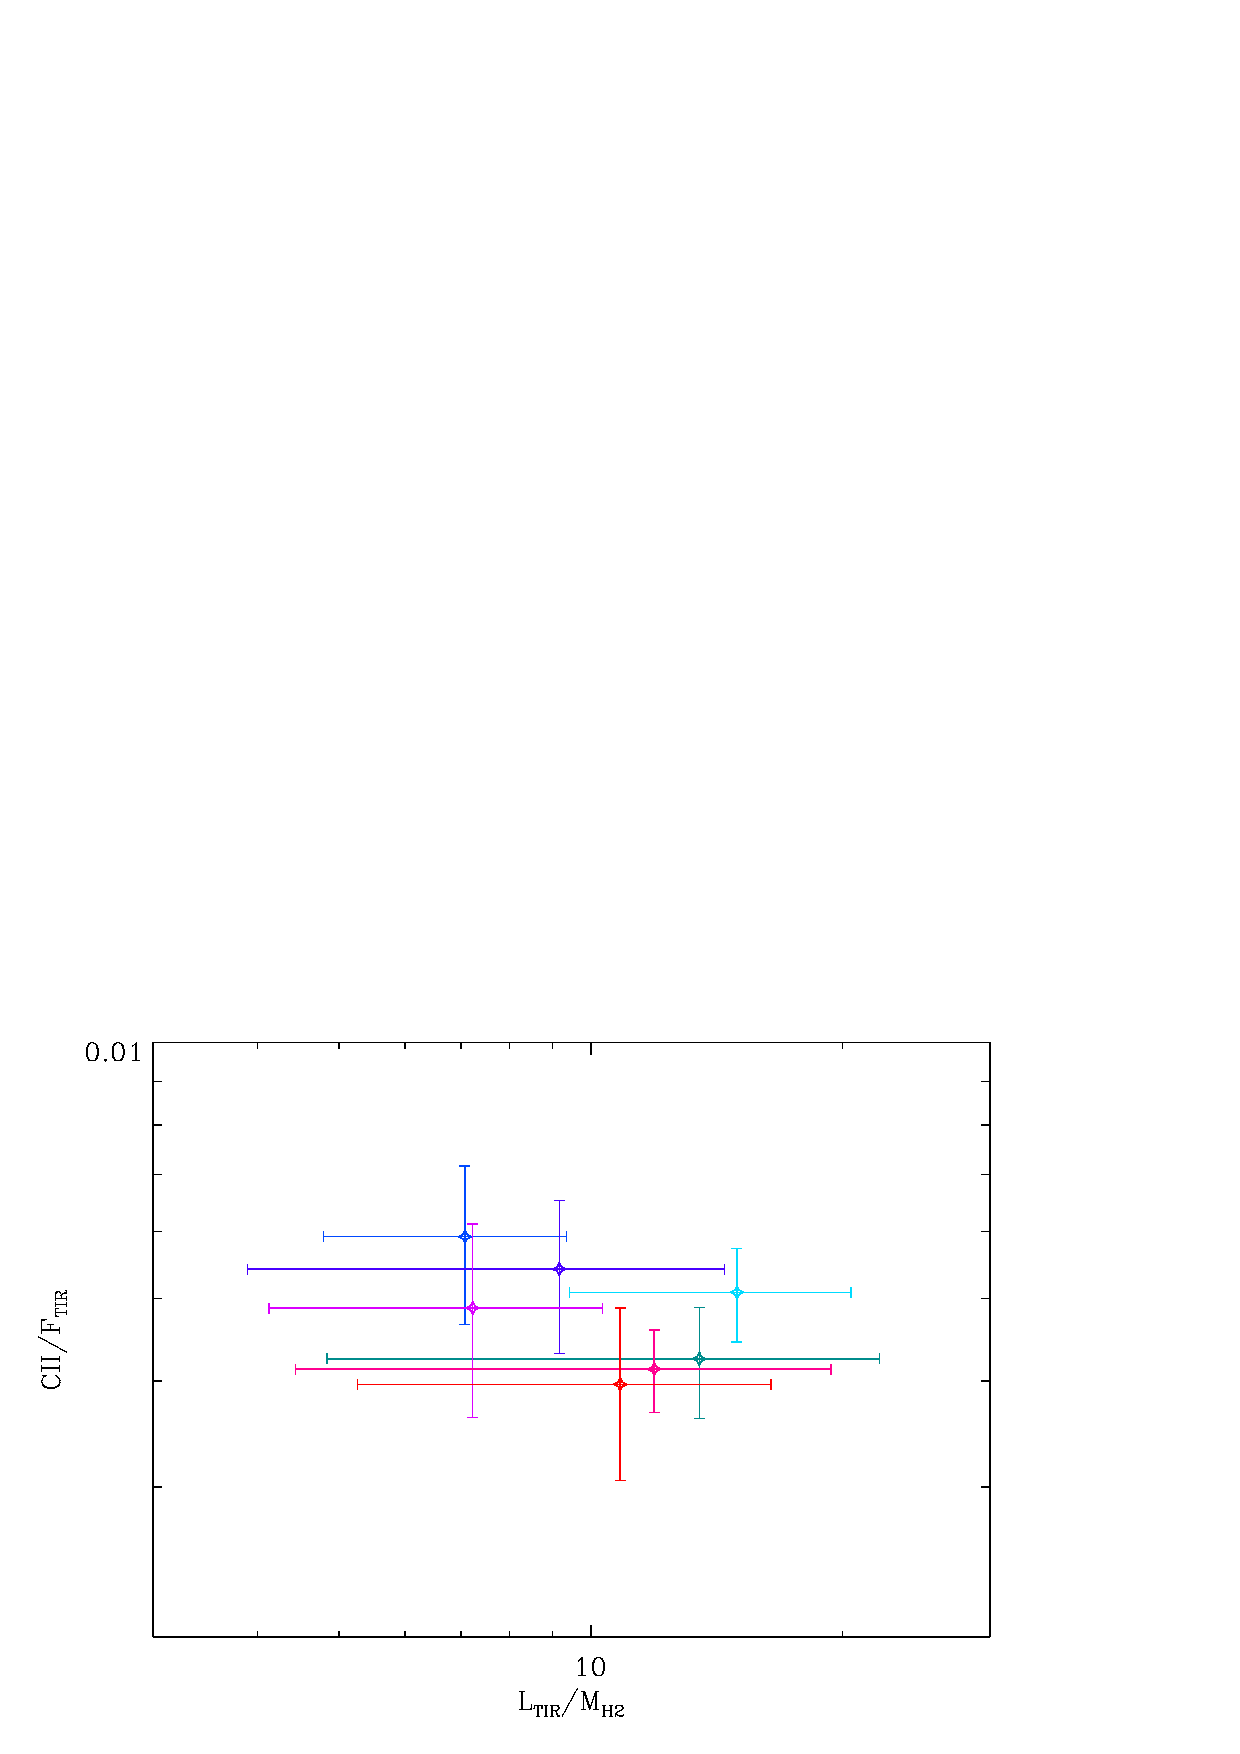
\includegraphics[width=\columnwidth]{CenA_CIIonFtir_LtironMH2_plot_v1}
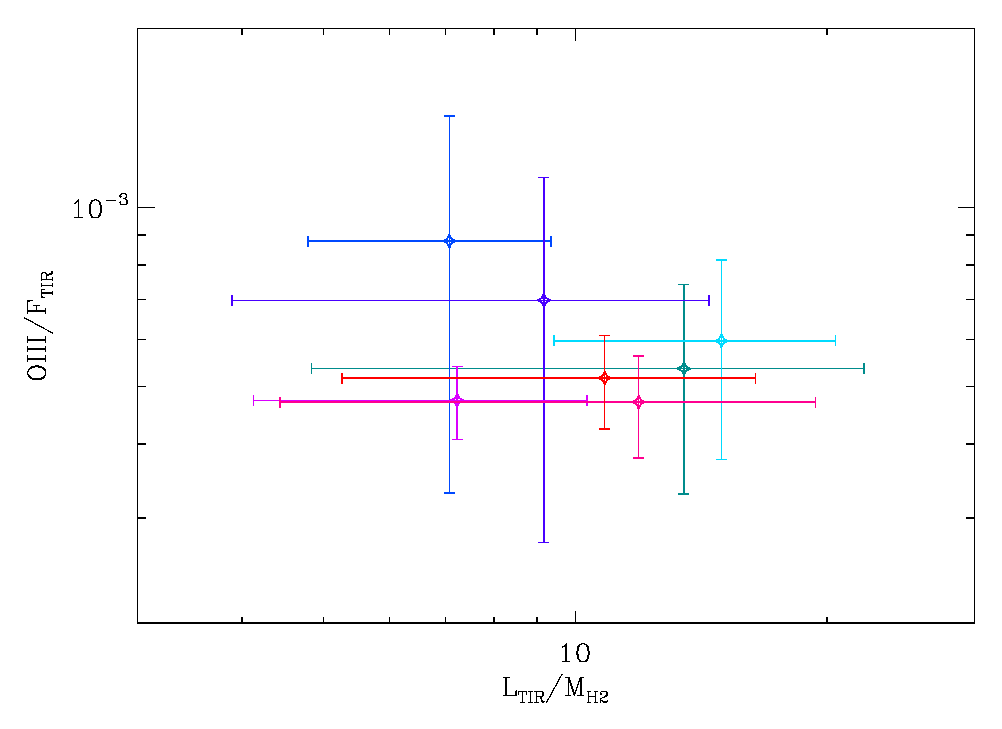
\includegraphics[width=\columnwidth]{CenA_OIIIonFtir_LtironMH2_plot_v1}
\caption{The [C~\textsc{ii}] (\emph{top}) and [O~\textsc{iii}] (\emph{bottom}) line ratios divided by the total infrared flux, $F_{\mathrm{TIR}}$ for Cen~A.  Each colored data point corresponds to a bin as described in Figure~\ref{fig:pdr_plots}.}
\label{fig:sfr}
\end{figure}

\subsubsection{Ionized Gas Source}\label{oiiionnii}
The observed [O~\textsc{iii}]$_{88}$/[N~\textsc{ii}]$_{122}$ line ratio has been used in high redshift sources to interpret either the strength of the ionization parameter, $U$, which is the number of ionizing photons divided by the gas density wthin the narrow line region of an AGN \citep{2009ApJ...701.1147A}, or the stellar classification of the youngest stars in an H~\textsc{ii} region, depending on the type of region one is investigating \citep{2011ApJ...740L..29F}.  We have taken the average observed [O~\textsc{iii}]/[N~\textsc{ii}]$_{122}$ and plotted it in Figure~\ref{fig:OIIIonNII} as a black dotted line, with the shaded region outlining the range of values within calibration uncertainties.  Overlaid on the observed ratio are four predicted line ratios as a function of stellar temperature from the H~\textsc{ii} region models of \citet{1985ApJS...57..349R} as shown by the dashed lines.  The various colors represent different gas densities.  Our results fall within a stellar effective temperature of approximately $3.45 \times 10^{4}$ and $3.62 \times 10^{4}$~K, which corresponds to stellar classifications of O9.5 or O9 \citep{1996ApJ...460..914V}.  The dash-dotted lines overlaid on the plot represent various narrow line region models from \citet{2004ApJS..153....9G}.  Comparing the range of our observations to the coinciding models we see that if the central AGN was influencing the surrounding gas out to the limits of our observations, the ionization parameter would range from log$U$ = -4 to -3.2, corresponding to a fairly weak AGN.  Given that we are not probing the AGN directly, it is more likely the [O~\textsc{iii}]$_{88}$/[N~\textsc{ii}]$_{122}$ line ratio is indicating that stars are producing the H~\textsc{ii} regions within our observations, or perhaps both the AGN and the stars.  If the AGN were to contribute partially to the observed emission it might explain why our observed [O~\textsc{iii}]$_{88}$/[N~\textsc{ii}]$_{122}$ line ratio is higher (and thus the stellar classification is earlier) than is observed in M51 \citep{parkin_2013}.

\begin{figure}
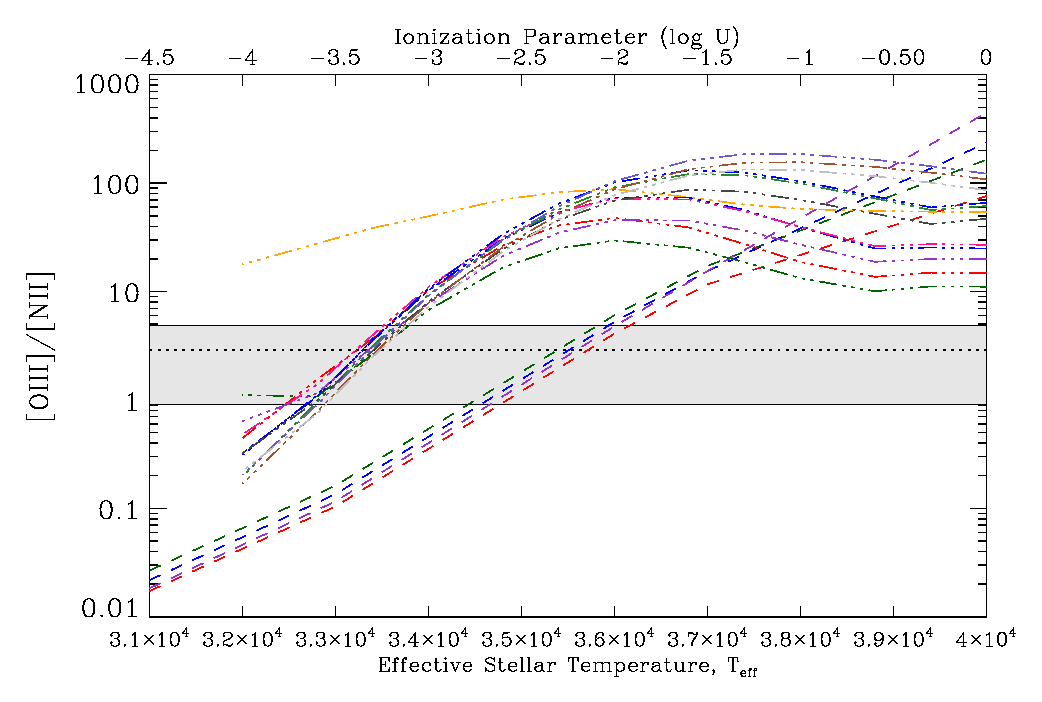
\includegraphics[width=\columnwidth]{CenA_OIIIonNII_plot_v2_cropped}
\caption{A comparison of the average observed [O~\textsc{iii}]$_{88}$/[N~\textsc{ii}]$_{122}$ line ratio for CenA to predicted line ratios for models of an H~\textsc{ii} region as well as a narrow line region AGN model. The black dotted line represents the global average over our observed line ratio, while the shaded region encompasses the range of values within uncertainty.  The dashed lines show the predicted line ratio as a function of effective stellar temperature (bottom axis) for various gas densities using the H~\textsc{ii} region model of \citet{1985ApJS...57..349R}.  The dash-dotted lines represent the predicted line ratios for the NLR regions as a function of the log of the ionization parameter $U$ (top axis) for various gas densities and power law indices using the model of \citet{2004ApJS..153....9G}.}
\label{fig:OIIIonNII}
\end{figure}

\subsection{The contribution of ionized gas to the [C~{\footnotesize II}] emission}\label{ion_gas}
The emission in the [C~\textsc{ii}]$_{158}$ line comes from three sources: dense neutral gas, ionized gas, and diffuse neutral gas.  For us to properly utilize the photodissociation region model in Section~\ref{pdr_model} to interpret our diagnostic far-infrared spectral lines, we need to isolate the [C~\textsc{ii}]$_{158}$ emission from the dense neutral gas found in PDRs.  The ionized gas contribution can be determined by comparing two observed line ratios, namely the [N~\textsc{ii}]$_{122}$/[N~\textsc{ii}]$_{205}$ and [C~\textsc{ii}]$_{158}$/[N~\textsc{ii}]$_{205}$ ratios to a theoretical prediction for each line as a function of electron density in an H~\textsc{ii} region \citep[e.g.][]{2006ApJ...652L.125O, parkin_2013}.  To calculate the level populations (and thus the predicted fluxes) for the two [N~\textsc{ii}] transitions we employ the Einstein coefficients from \citet{1997A&AS..123..159G} and collision strengths from \citet{2004MNRAS.348.1275H}.  For the [C~\textsc{ii}]$_{158}$ line level populations we use the Einstein coefficients of \citet{1998A&AS..131..499G} and collisions strengths of 
\citet{1992ApJS...80..425B}.  Due to the lack of accurate measurements of the gas phase abundances of C or N, as well as the metallicity in Cen~A, we adopt Solar gas phase abundances and assume no metallicity gradient within the region we are investigating.   The abundances we choose are from \citet{1996ARA&A..34..279S}, and are C/H~$= 1.4 \times 10^{-4}$ and N/H~$= 7.9 \times 10^{-5}$.

%The theoretical curves for the [N~\textsc{ii}]$_{122}$/[N~\textsc{ii}]$_{205}$ and %[C~\textsc{ii}]$_{158}$/[N~\textsc{ii}]$_{205}$ line ratios are shown in %Figure~\ref{fig:ion_plot}.

%\begin{figure}
%\includegraphics[width=7.5cm]{CenA_I122onI205_plot}
%\caption{Theoretical curves for the [N~\textsc{ii}]$_{122}$/[N~\textsc{ii}]$_{205}$ and %[C~\textsc{ii}]$_{158}$/[N~\textsc{ii}]$_{205}$ line ratios as a function of electron %density in ionized gas, shown as the solid and dashed lines, respectively.}
%\label{fig:ion_plot}
%\end{figure}

Our observed [N~\textsc{ii}]$_{122}$/[N~\textsc{ii}]$_{205}$ line ratio is initially calculated for the small region of overlap between the observations of the two lines.  We convolve the [N~\textsc{ii}]$_{122}$ to the resolution of the [N~\textsc{ii}]$_{205}$ ($17\arcsec$) and align the two maps and regrid to a common pixel scale.  Next, we convert the units of the [N~\textsc{ii}]$_{122}$ map to match those of the [N~\textsc{ii}]$_{205}$, Jy~beam$^{-1}$, and then calculate the line ratio in each of the overlapping pixels.  We follow the same steps in producing the [C~\textsc{ii}]$_{158}$/[N~\textsc{ii}]$_{205}$ line ratio.

Using theoretical curves of the line ratios as a function of electron density for an H~\textsc{ii} region, we determine the electron density at which our observed [N~\textsc{ii}]$_{122}$/[N~\textsc{ii}]$_{205}$ ratio matches that of the theoretical prediction for each pixel.  We find a mean electron density of 6.3~cm$^{-3}$ with lower and upper limits of 0.8 and 12.3~cm$^{-3}$.  Given that there is little overlap between our [N~\textsc{ii}]$_{205}$ map and our [N~\textsc{ii}]$_{122}$ map, we choose to take the mean observed ratio and standard deviation as the adopted [N~\textsc{ii}]$_{122}$/[N~\textsc{ii}]$_{205}$ measurement for the full area of our PACS observations.  Thus, we find [N~\textsc{ii}]$_{122}$/[N~\textsc{ii}]$_{205} = 0.8 \pm 0.2$, and create an [N~\textsc{ii}]$_{205}$ map that we can then, in turn, use to create an observed [C~\textsc{ii}]$_{158}$/[N~\textsc{ii}]$_{205}$ map.

With the electron density known, we then determine the theoretical prediction for the [C~\textsc{ii}]$_{158}$/[N~\textsc{ii}]$_{205}$ ratio in the ionized gas.  Dividing the predicted ratio map by our observed ratio map provides us with the fraction of [C~\textsc{ii}] emission originating in H~\textsc{ii} regions.  This is then subtracted from our [C~\textsc{ii}]$_{158}$ map.  In Figure~\ref{fig:cii_ion_map} we show the fraction of [C~\textsc{ii}]$_{158}$ emission coming from ionized gas along the disk of Cen~A covered by our observations.

\begin{figure}
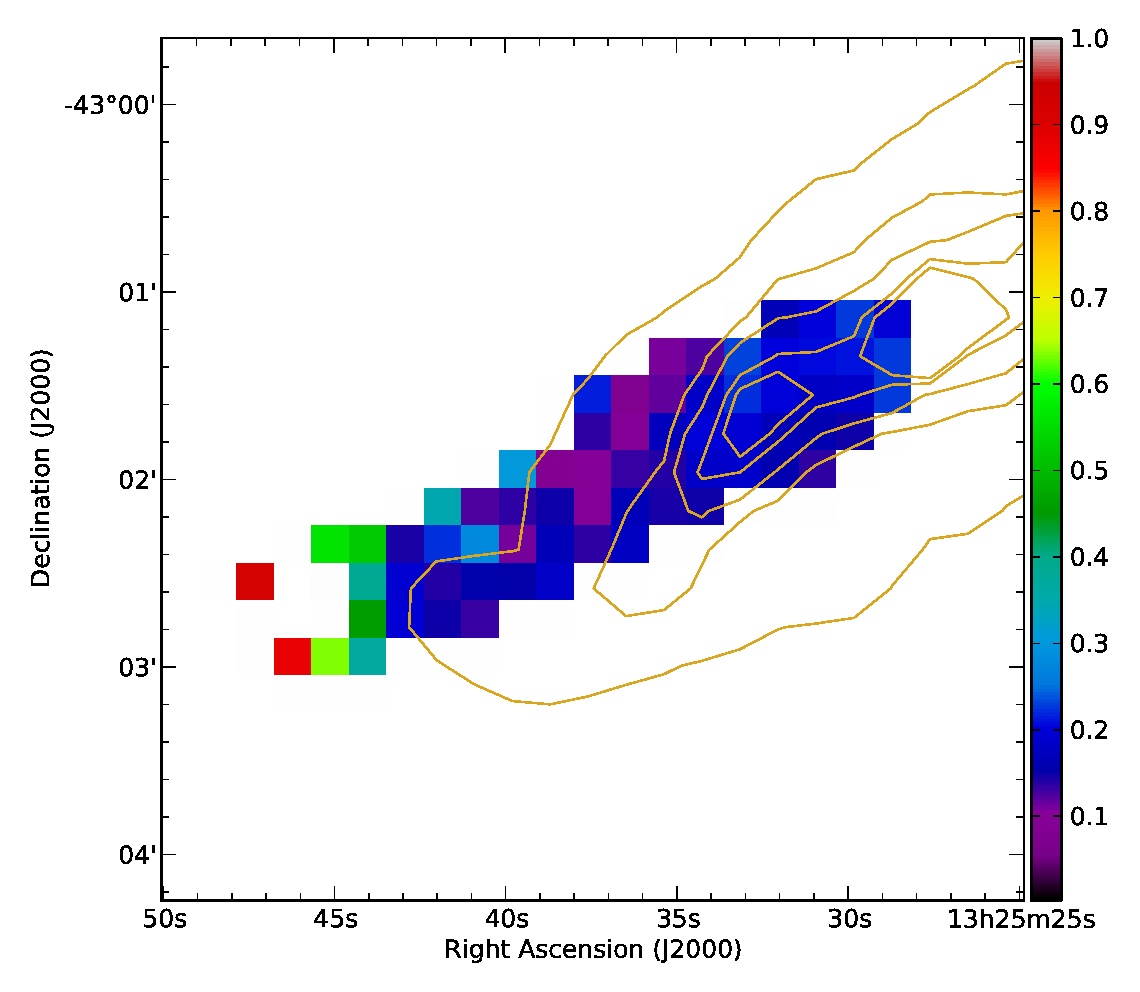
\includegraphics[width=\columnwidth]{CenA_ion_fraction}
\caption{The fraction of [C~\textsc{ii}]$_{158}$ emission originating from ionized gas for the eastern half of the disk of Centaurus~A.}
\label{fig:cii_ion_map}
\end{figure}

For comparison with the PDR model in Section~\ref{pdr_model}, we remove the fraction of [C~\textsc{ii}]$_{158}$ emission coming from ionized gas, which in general is quite low.  The majority of our map demonstrates a contribution of roughly 10 to 20\%, with the pixels showing the highest ionized gas contribution falling at the edge of the map farthest from the center of the galaxy, where the signal-to-noise is lower.


%%%%%%%%%%%%%%%%%%%%%%%%%%%%%%%%%%%%%%%%%%%%%%%%%%%%%%%%%%%%%
\section{PDR modelling}\label{pdr_model}

A comparison between observed line ratios and a PDR model allows us to diagnose the physical properties of the molecular clouds from which the fine structure line emission originates.  Here we choose to use the PDR model of \citet{1999ApJ...527..795K,2006ApJ...644..283K}, which has been updated and expanded from the model of \citet{1985ApJ...291..722T}.  This particular model assumes the PDR is a plane-parallel, semi-infinite slab and is only parameterized by two free variables: the hydrogen gas density, $n$, and the strength of the impeding far-ultraviolet (FUV) radiation field normalized to the Habing field \citep[$1.6 \times 10^{-3}$~erg~cm$^{-2}$~s$^{-1}$; ][]{1968BAN....19..421H}, $G_{0}$.  The model simultaneously treats the thermal balance, chemical network and radiative transfer and produces a grid of predicted fine structure line strengths as a function of $n$ and $G_{0}$.  By comparing observed line ratios to the predicted ones we can extract the corresponding $n$ and $G_{0}$.

For our investigation we choose to utilize the line ratio parameter space of [C~\textsc{ii}]$_{158}$/[O~\textsc{i}]$_{63}$ vs. [C~\textsc{ii}]$_{158}$+[O~\textsc{i}]$_{63}$)/$F_{\mathrm{TIR}}$.  In order to search for radial variations in the disk of Cen~A we have divided our observed line ratio maps into eight bins of pixels to measure $n$ and $G_{0}$.  The area of our line ratio maps is displayed in the top left panel of Figure~\ref{fig:pdr_plots}, where the bins are color-coded and labelled.  The average observed values in each bin are overlaid on the PDR model grid in the top right panel of Figure~\ref{fig:pdr_plots}, with the error bars incorporating both the measurement and calibration uncertainties of the observations as well as the standard deviation of the data in each bin.  We note here that the total infrared flux, $F_{\mathrm{TIR}}$, has been reduced by a factor of two as recommended by \citet{1999ApJ...527..795K} to accommodate the fact that the observed total flux emits from both the near and far sides of the cloud(s) because it is optically thin; however, the model assumes it only emits from the side exposed to the source of FUV flux.  The resulting values of $n$, $G_{0}$ and the temperature at the surface of the PDR, $T$, are presented in Table~\ref{table:cena_pdr_model_results} under the ``Uncorrected" heading.

The PDR model assumes the [C~\textsc{ii}]$_{158}$ emission originates only in neutral gas, but as described in Section~\ref{ion_gas}, [C~\textsc{ii}]$_{158}$ emission can be produced in both neutral and ionized gas.  Thus, to properly compare our observations to the model we need to remove the contribution from the ionized gas.  We also need to make a correction to the [O~\textsc{i}]$_{63}$ observations that stems from geometrical effects of many PDRs in a given observation for extragalactic sources.  We see PDRs at all orientations with respect to our line of sight, but observed emission only escapes from the lit side of the PDR when the line is optically thick, as is the case for the [O~\textsc{i}]$_{63}$ line.  \citet{1999ApJ...527..795K} state that as a result of the optically thick line and various PDR orientations, we only observe about half of the total [O~\textsc{i}]$_{63}$ emission produced, while the remaining half radiates away from the line of sight.  Thus, we opt to follow this advice and increase our observed [O~\textsc{i}]$_{63}$ flux by a factor of 2, as we have previously done with M51 \citep{parkin_2013}.  We show the fully corrected line ratios compared to the PDR model in the bottom left panel of Figure~\ref{fig:pdr_plots} and tabulate the results in Table~\ref{table:cena_pdr_model_results}.  We see that with these changes the data points shift down and slightly to the right, corresponding to increases in both $G_{0}$ and $n$.

As a consistency check, in Figure~\ref{fig:pdr_plots} (bottom right panel) we also show a comparison of our observations with the PDR model parameter space [C~\textsc{ii}]/[O~\textsc{i}]$_{145}$ vs. ([C~\textsc{ii}]+[O~\textsc{i}]$_{63}$)/$F_{\mathrm{TIR}}$, which has the advantage of the optically thin [O~\textsc{i}]$_{145}$ line.  We find that this parameter space gives consistent solutions for $n$ and $G_{0}$ as those derived from the plot in the bottom left panel of the same figure.  This reassures us that our assumption that the [O~\textsc{i}]$_{63}$ line is optically thick is valid.

\begin{figure*}
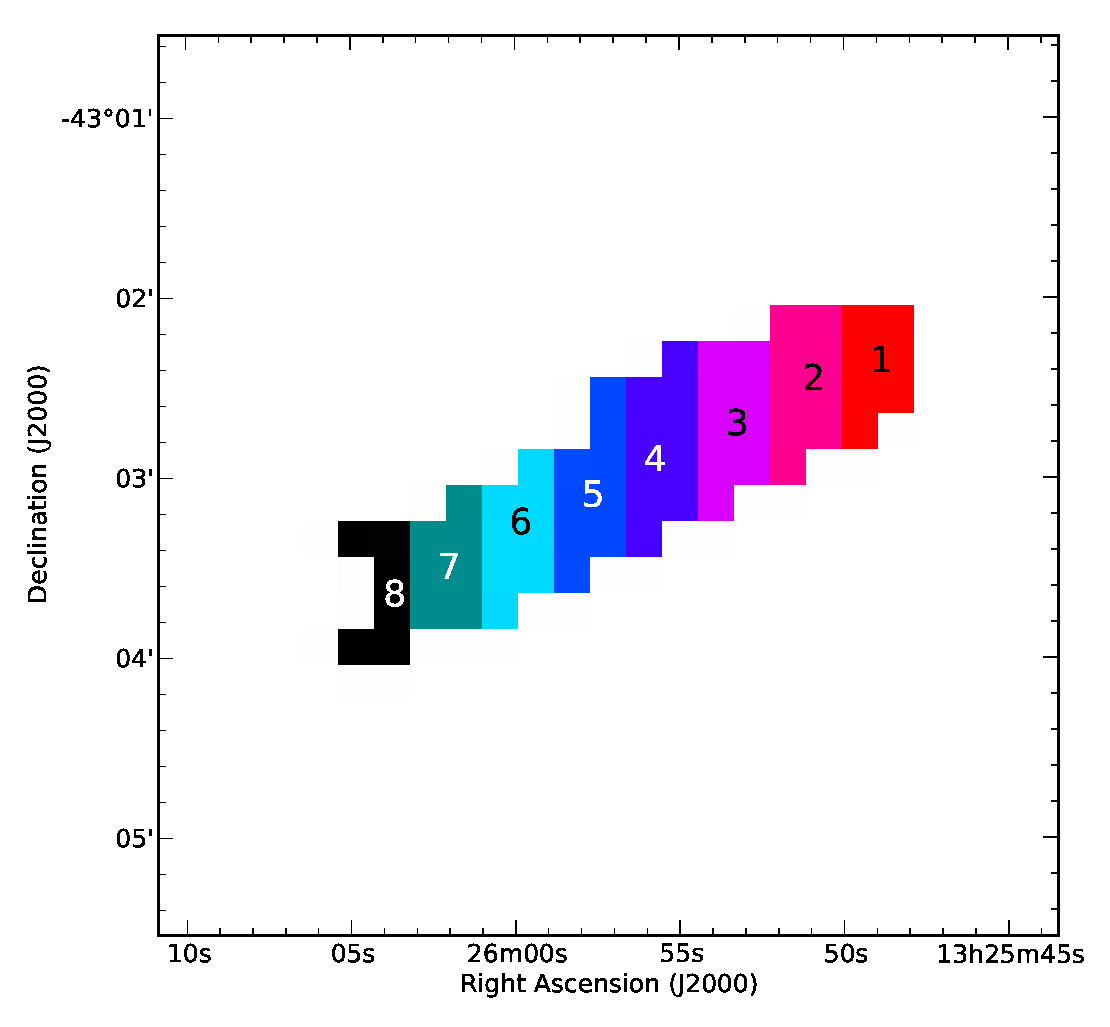
\includegraphics[width=\columnwidth]{CenA_colour_guide_cropped}
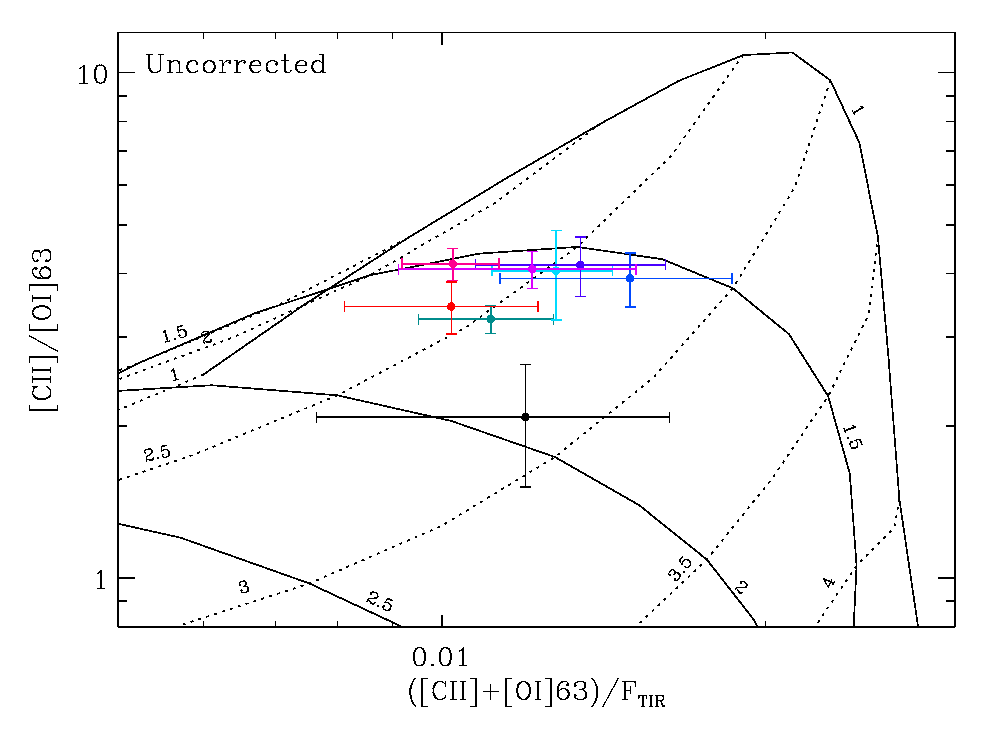
\includegraphics[width=\columnwidth]{CenA_CIIOI63_vs_CIIOI63onFtir_uncorrected_plot_radial_bins_v2}
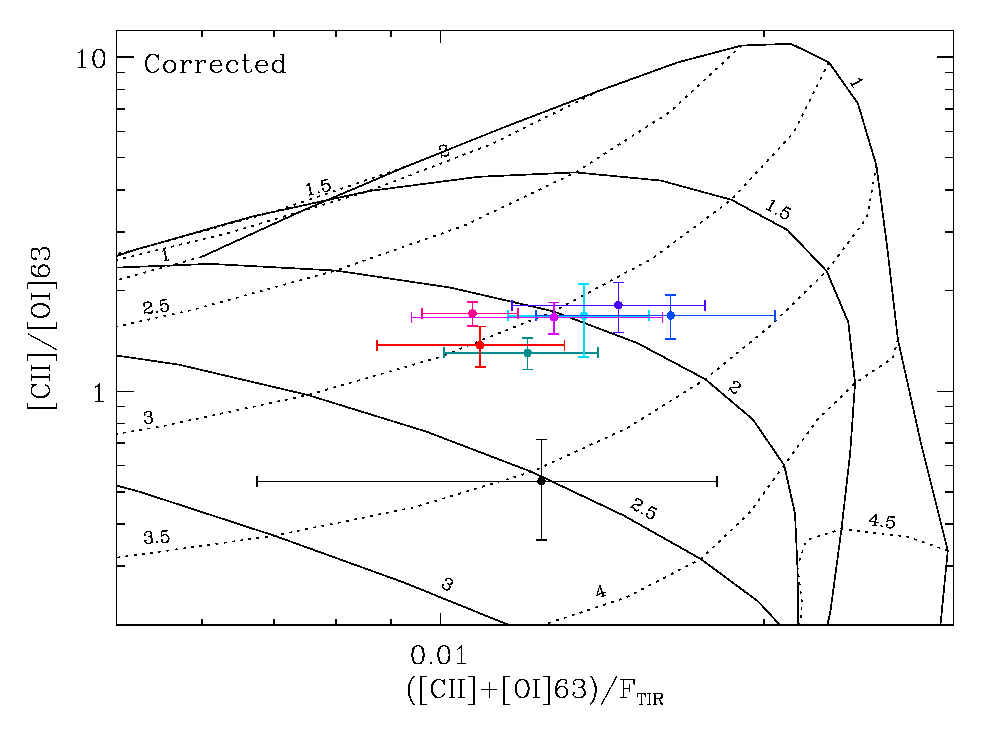
\includegraphics[width=\columnwidth]{CenA_CIIOI63_vs_CIIOI63onFtir_corrected_plot_radial_bins_v2}
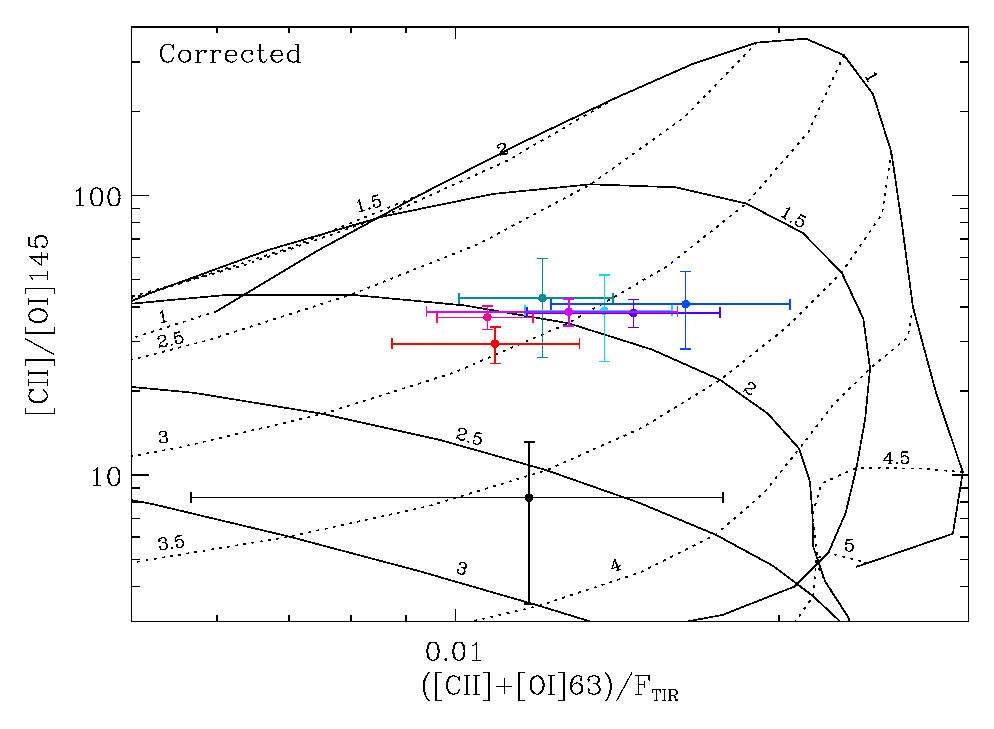
\includegraphics[width=\columnwidth]{CenA_CIIOI145_vs_CIIOI63onFtir_corrected_plot_radial_bins_v2}
\caption{\emph{top left}: A schematic of the radial bins we divide our observed line ratio maps into.  The colors in this image correspond to the data points in the other three panels of this figure. \emph{top right}: A comparison of our observed (and uncorrected) [C~\textsc{ii}]/[O~\textsc{i}]$_{63}$ and ([C~\textsc{ii}]+[O~\textsc{i}]$_{63}$)/$F_{\mathrm{TIR}}$ line ratios to the PDR model of \citet{1999ApJ...527..795K} for the eastern half of Centaurus~A. The data points represent our observations, each color corresponding to a radial bin as shown in the top left panel.  The solid lines represent contours of constant log$G_{0}$ while the dotted lines represent curves of constant log$n$.  \emph{bottom left}: The same plot as in the top right panel, but here the [C~\textsc{ii}] and [O~\textsc{i}]$_{63}$ have been corrected as described in the text. \emph{bottom right}: Our observed [C~\textsc{ii}]/[O~\textsc{i}]$_{145}$ and ([C~\textsc{ii}]+[O~\textsc{i}]$_{63}$)/$F_{\mathrm{TIR}}$ line ratios compared to the PDR model.  The lines and data points are the same as in the top right and bottom left panels.}
\label{fig:pdr_plots}
\end{figure*}

\begin{deluxetable}{lccccc}
\tabletypesize{\small}
\tablecolumns{5}
\tablecaption{Properties of the gas derived from the PDR model\label{table:cena_pdr_model_results}}
\tablewidth{0pt}
\tablehead{
\colhead{Case}
 & \colhead{Bin} & \colhead{log($n$/cm$^{-3}$)} & \colhead{log$G_{0}$}
	& \colhead{$T$ (K)}}
 \startdata
 uncorrected\tablenotemark{a}
 & 1 & (2.25--2.5)$^{+0.5}_{-0.75}$ & (1.5--1.75)$^{+0.5}_{-0.25}$
 	& (120--170)$^{+655}_{-40}$ \\
 & 2 & (2.0--2.25)$^{+0.5}_{-0.5}$  & (1.5--1.75)$^{+0.25}_{-0.5}$
 	& (140--210)$^{+410}_{-70}$ \\
 & 3 & (2.25--2.5)$^{+0.5}_{-0.75}$ & (1.5--1.75)$^{+0.25}_{-0.25}$
 	& (120--170)$^{+450}_{-40}$ \\
 & 4 & (2.5--2.75)$^{+0.5}_{-1.0}$  & (1.5--1.75)$^{+0.25}_{-0.25}$
 	& (110--150)$^{+470}_{-35}$ \\
 & 5 & (2.5--2.75)$^{+0.5}_{-1.0}$  & (1.5--1.75)$^{+0.25}_{-0.25}$
 	& (110--150)$^{+470}_{-35}$ \\
 & 6 & (2.5--2.75)$^{+0.25}_{-1.0}$ & (1.5--1.75)$^{+0.25}_{-0.25}$
 	& (110--150)$^{+470}_{-30}$ \\
 & 7 & (2.5--2.75)$^{+0.25}_{-1.0}$ & (1.5--1.75)$^{+0.25}_{-0.25}$
 	& (110--150)$^{+470}_{-30}$ \\
 & 8 & (2.75--3.0)$^{+0.5}_{-0.5}$  & (1.75--2.0)$^{+0.25}_{-0.25}$
 	& (130--170)$^{+85}_{-40}$ \\
 \hline
 corrected\tablenotemark{b}
 & 1 & (3.0--3.25)$^{+0.25}_{-0.5}$  & (2.0--2.25)$^{+0.25}_{-0.25}$
 	& (155--200)$^{+70}_{-40}$ \\
 & 2 & (2.75--3.0)$^{+0.25}_{-0.25}$ & (2.0--2.25)$^{+0.25}_{-0.25}$
 	& (160--200)$^{+70}_{-35}$ \\
 & 3 & (3.0--3.25)$^{+0.25}_{-0.5}$  & (2.0--2.25)$^{+0.25}_{-0.25}$
 	& (155--200)$^{+70}_{-40}$ \\
 & 4 & (3.0--3.25)$^{+0.5}_{-0.5}$   & (1.75--2.0)$^{+0.25}_{-0.25}$
 	& (125--160)$^{+60}_{-45}$ \\
 & 5 & (3.0--3.25)$^{+0.5}_{-0.25}$  & (1.75--2.0)$^{+0.25}_{-0.5}$
 	& (125--160)$^{+40}_{-55}$ \\
 & 6 & (3.0--3.25)$^{+0.25}_{-0.5}$  & (1.75--2.0)$^{+0.25}_{-0.0}$
 	& (125--160)$^{+60}_{-10}$ \\
 & 7 & (3.0--3.25)$^{+0.25}_{-0.25}$ & (2.0--2.25)$^{+0.25}_{-0.25}$
 	& (155--200)$^{+50}_{-40}$ \\
 & 8 & (3.5--3.75)$^{+0.25}_{-0.5}$  & (2.5--2.75)$^{+0.5}_{-0.5}$
 	& (200--260)$^{+110}_{-90}$ \\
 \enddata
 \tablecomments{The values reported for log$G_{0}$, log($n$/cm$^{-3}$), and T show the best fitting range from the model grid in brackets.  The lower limits on these values are calculated by subtracting the lower uncertainty from the lower end of the best fitting range, while the upper limits should be calculated by adding the upper uncertainty to the upper end of the best fitting range.}
 \tablenotetext{a}{The uncorrected results include all of the observed [C~\textsc{ii}] emission.}
 \tablenotetext{b}{The corrected results include only [C~\textsc{ii}] emission from neutral gas, and the [O~\textsc{i}]63 has been increased by a factor of two to account for multiple PDRs.}
\end{deluxetable}

We note here that there is a second solution in this parameter space which diagnoses the molecular clouds with a weaker $G_{0}$ ($\sim 10^{0}-10^{0.75}$)and higher $n$ ($\sim 10^{3.5}-10^{4.25}$).  However, comparing our observed [C~\textsc{ii}] integrated intensity to that the predicted by the PDR model based on the second solution, the second solution would suggest that there are up to a few thousand PDRs along each line of sight, which, despite the fact that Cen~A is almost edge on, seems unlikely within a 14$\arcsec$ beam.  A similar argument has been used by \citet{2005A&A...441..961K} and \citet{parkin_2013} to infer that this solution is invalid.  Thus, we eliminate this solution for the discussion aspects of this paper.

%%%%%%%%%%%%%%%%%%%%%%%%%%%%%%%%%%%%%%%%%%%

\section{Discussion}\label{discussion}
%\subsection{Role of the AGN}\label{agn_role}
The heating efficiency and [C~\textsc{ii}]/$F_{\mathrm{TIR}}$ line ratios found along the strip of Cen~A are consistent with values found in other normal, star forming spiral galaxies as was discussed above in Section~\ref{subsec:ratio}, with an average value of $(6 \pm 2) \times 10^{-3}$.  We also see, for the first time, a slight decrease in efficiency toward the center of the galaxy, which tells us the dust grains and PAHs that provide the free electrons for gas heating are likely becoming too positively charged for the photoelectric effect to take place efficiently.  The most likely cause of the heating deficiency is the AGN itself, as it would generate a hard radiation field.  We do see support for this in Figure~\ref{fig:pacs_spec_maps} in the [O~\textsc{iii}] and [N~\textsc{ii}]$_{122}$ lines, which show peaked emission near the edge of our observations toward the center of the galaxy.  We also see strong [N~\textsc{ii}]$_{205}$ emission in the nucleus of the galaxy.  In contrast, we also see the strongest [O~\textsc{i}]$_{63}$ emission toward the center of the galaxy, indicating the presence of neutral gas.  However, this line can also be indicative of gas heating via shocks \citep{1989ApJ...342..306H}.

In \citet{2012MNRAS.422.2291P} a radially decreasing trend in both the dust temperature and the gas-to-dust mass ratio was reported, implying some influence on the surrounding ISM by the central AGN in Cen~A.  Interestingly, we do not see a radial trend in the density of hydrogen nuclei, $n$ nor the strength of the interstellar radiation field impeding onto the molecular cloud surfaces $G_{0}$, within the combined statistical plus calibration uncertainties (shown in Figure~\ref{fig:pdr_plots}).  Even within one standard deviation of the mean value in each bin (not shown), there is little trend with increasing radius from the center (only the outermost bin shows a significant deviation from the other bins; however, this may be due low signal-to-noise in the pixels).  Correspondingly, the surface temperature of the clouds also does not show a radial trend, in contrast to the dust temperature.  These results suggest that the physical properties of the molecular clouds nearest the center in our observations are not being affected strongly by the AGN.

One possible explanation for this might be the high inclination of Cen~A with respect to the line of sight.  Cen~A has an inclination of roughly 75$^{\circ}$ \citep{2006ApJ...645.1092Q} so it is nearly edge on.  If we were only diagnosing the characteristics of clouds from the nearest side of the galaxy, we might not observe any effects of the AGN on the surrounding clouds.  However, while we believe the [O~\textsc{i}]$_{63}$ line is optically thick, [O~\textsc{i}]$_{145}$ is not, and it is unlikely the [C~\textsc{ii}], and $F_{\mathrm{TIR}}$ are optically thick as well.  Thus, it is more likely that any effects the AGN might have on the surrounding gas are diluted because we are integrating emission over clouds through the arm and interarm regions as well as any in the vicinity of the AGN along our line of sight.

Another possibility to explain why the dust, tracing the inner parts of giant molecular clouds (GMCs) and the diffuse ISM, is affected by the AGN but not the PDR gas, is that the AGN is affecting these regions of the ISM more so than around the edges of GMCs, where warm PDRs tend to exist due to recent massive star formation.  This might be plausible if the X-rays produced by the AGN are affecting the diffuse ISM more than the PDRs, and an appreciable fraction of the observed dust continuum is from the diffuse ISM.

We also note that the dust temperatures are colder (20--30~K) than those in the gas (roughly 100-300~K).  This may not be surprising, as the far-infrared continuum is optically thin and thus we are probing deeper into the cloud, whereas the PDR model only provides us with the temperature of the gas at the surface.  Furthermore,  \citet{2012MNRAS.422.2291P} fit the dust SED between 70 and 500~$\mu$m where the dust grains are more likely to be in thermal equilibrium with their surroundings, while the hotter dust grains would be better represented by mid-infrared continuum, such as at 24~$\mu$m map, which is often used as an obscured star formation tracer \citep{2005ApJ...632L..79W, 2007ApJ...666..870C, 2010ApJ...714.1256C, 2009ApJ...703.1672K}.


\subsection{Inferred Physical Conditions from PDR Modelling}\label{discuss_pdr}
In Section~\ref{pdr_model} we found that the average values of $G_{0}$ and $n$ across the disk ranged from $\sim 10^{1.75}$--10$^{2.75}$ and $\sim 10^{2.75}$--$10^{3.75}$~cm$^{-3}$, respectively.  These results are consistent with those previously published by \citet{2000A&A...355..885U}, who found $G_{0} \sim 10^{2}$ and $n \sim 10^{3}$~cm$^{-3}$, as well as by \citet{2001A&A...375..566N} who found $G_{0} = 10^{2.7}$ and $n = 10^{3.1}$~cm$^{-3}$ for Cen~A.  The properties of the molecular clouds are also consistent with those found by large surveys on global scales.  The 60 galaxies in the \citet{2001ApJ...561..766M} sample show $10^{2} \le G_{0} \le 10^{4.5}$ and $10^{2}\,\mathrm{cm}^{-3} \le n \le 10^{4.5}\,\mathrm{cm}^{-3}$, while the full sample of \citet{2001A&A...375..566N} shows a range of 10$^{2}$ to 10$^{4}$ for both $n$ and $G_{0}$, where $n$ is in units of cm$^{-3}$.  

We also compare our results to those found for other individual galaxies.  \citet{2013A&A...549A.118C} investigated the PDR characteristics within four regions of the starbust M82.  They found that within their central starbust and disk components, $G_{0} = 2500$, $n = 900$~cm$^{-3}$, and $G_{0} = 450$, $n = 220$~cm$^{-3}$, respectively, consistent with the results for Cen~A.  \citet{2012ApJ...747...81C} found values for $G_{0}$ and $n$ of 10$^{1.7}$--10$^{3.0}$ and 10$^{2.5}$--10$^{3.0}$~cm$^{-3}$ for the Seyfert~1 galaxy NGC~1097 and the spiral galaxy NGC~4559, while \citet{2002AJ....124..751C} found values of $G_{0}$ and $n$ of $10^{2.0}$--10$^{4.0}$  and $10^{2.0}$--10$^{4.0}$~cm$^{-3}$ for the two spiral galaxies NGC~6946 and NGC~1313.  Lastly, in M33, a nearby spiral, \citet{2011A&A...532A.152M} find $G_{0} = 32$ and $n = 320$~cm$^{-3}$.  Thus, Cen~A has a lower value for $G_{0}$ for M82, but a higher value for $G_{0}$ than M33, and is in fairly good agreement with the range of values of $G_{0}$ and $n$ found in other sources.

In contrast to the values for $G_{0}$ and $n$ found in normal or starbursting galaxies, Wilson et al. (in prep) investigated the elliptical galaxy NGC~4125 and found that the [C~\textsc{ii}]/[O~\textsc{i}]$_{63}$ line ratio is greater than 3--4 (including calibration uncertainties) and ([C~\textsc{ii}]+[O~\textsc{i}]$_{63}$)/$F_{\mathrm{TIR}}$ is greater than $1.3 \times 10^{-3}$.  These values would place it left and upwards in the parameter space in the top right panel of Figure~\ref{fig:pdr_plots}, in a region where only the low $G_{0}$, high $n$ solutions lie (not shown in the figure).  We choose to compare these line ratios for NGC~4125 with our uncorrected results for Cen~A because the [C~\textsc{ii}] emission from NGC~4125 was not corrected for ionized gas.  In fact, it is likely that NGC~4125 is ionized gas dominated given that only an upper limit for [O~\textsc{i} ]$_{63}$ is determined but there are significant detections in [N~\textsc{ii}]$_{122}$ and [C~\textsc{ii}].  Furthermore, \citet{2010ApJ...725..100W} find only an upper limit in CO emission for NGC4125.

\citet{2011MNRAS.410.1197C} studied 12 early type galaxies and found their star forming properties to be similar to other star forming galaxies.  \citet{2012MNRAS.421.1298C} studied a subsample of early type galaxies from the ATLAS$^{3\mathrm{D}}$ survey \citep{2011MNRAS.414..940Y} and found diagnostic CO line ratios in many of these galaxies that were consistent with those of typical spiral galaxies.   Thus, Cen~A likely has a more normal ISM than NGC~4125 when compared to samples of elliptical and lenticular galaxies, as well as spiral galaxies.  

\subsection{Potential Non-PDR contributions to observed lines}
We note that there is a possibility that of the [C~\textsc{ii}] emission stemming from neutral gas, some may come from the diffuse ISM rather than from PDRs.  If this were the case, the data points in Figure~\ref{fig:pdr_plots} would shift downward and to the left.  However, \citet{2000A&A...355..885U} looked into this possibility and concluded that less than 5\% of the [C~\textsc{ii}] emission originated in non-PDR gas within their ISO observations of Cen~A.  Furthermore, we calculate the ratio of H$_{2}$/H~\textsc{i} using the maps from \citet{2012MNRAS.422.2291P} and find an average value of roughly 5 through the area covered by our spectroscopic strips, suggesting that the gas is molecular H$_{2}$ dominated.

In addition, it is possible that not all of the observed $F_{\mathrm{TIR}}$ emission stems from PDRs as well; for example, it could come from H~\textsc{ii} regions.  Looking at the right panel of Figure~\ref{fig:pdr_plots} we see that we can reduce the $F_{\mathrm{TIR}}$ by roughly a factor of 3 before our data become inconsistent with the PDR model.  Thus, at least 1/6 (the extra factor of two comes from the fact that we have already reduced the observed flux for comparison with the PDR) of the observed $F_{\mathrm{TIR}}$ emission in Cen~A comes from PDR gas.

\subsection{Comparison to M51}\label{compare_m51}
\citet{parkin_2013} investigated the same atomic fine structure lines in central $\sim2.5\arcmin$ of M51 by dividing the galaxy into four distinct regions: the nucleus, center, arm and interarm regions.  They discovered a radial trend in both the fraction of ionized gas (from about 80\% in the central region of the galaxy down to 50\% in spiral arm and interarm regions) as well as in the properties of the molecular clouds, $n$, $G_{0}$ and $T$.  However, they also discovered that in addition to the radial trend, the molecular clouds in the arm and interarm regions displayed the same physical characteristics, despite differing star formation rate surface densities.  We now discuss the similarities and differences between the properties of the gas in both M51 and Cen~A.

To give any meaning to this comparison we first need to consider the star formation rate (SFR) and star formation rate surface density (SFRD), $\Sigma(70)$.  We estimate the SFR of Cen~A by using the equation derived empirically by \citet{2013ApJ...768..180L} that uses the luminosity of the \emph{Herschel} PACS 70~$\mu$m map (their equation~(4), with the calibration constant determined for their combined dataset as listed in their Table~5):
\begin{equation}\label{eqn:sfr}
\mathrm{SFR}(70) = 1.18 \times 10^{-43} L(70),
\end{equation}
where the SFR rate is given in M$_{\odot}$~yr$^{-1}$ and the luminosity at 70~$\mu$m is given in erg~s$^{-1}$.  With this equation we obtain a total SFR in the region covered by our 70~$\mu$m map of approximately 3.7~M$_{\odot}$~yr$^{-1}$.   \citet{2013ApJ...768..180L} caution that the SFR determined with this equation for regions larger than approximately 200~pc may be overestimated by up to 50\% because Equation~\ref{eqn:sfr} assumes that $L(70)$ is entirely associated with recent star formation activity.  However, on scales larger than 200~pc diffuse 70~$\mu$m emission may account for half of the observed luminosity.  Each pixel in our 70~$\mu$m map has a 12$\arcsec$ scale, corresponding to a physical size of roughly 220~pc, at the limit of scale the equation is valid for.  However, since we are summing over the disk to obtain the total SFR, we will conservatively assume half of the 70~$\mu$m is not associated with current star formation, reducing the observed SFR to $\sim1.85$.

Next we need to estimate the SFRD for Cen~A.  Since it is edge on, while M51 is face on, we want to determine the area of the disk of Cen~A if it were face-on, as well.  For simplicity, we assume the disk is circular and take the radius to be that of the edge-on disk.  Given the warped nature of the disk we take two radius measurements as lower and upper bounds (3.5--6$\arcmin$), corresponding to upper and lower limits on the SFRD of $\Sigma(70) = 0.014$--$0.04$~M$_{\odot}$~yr$^{-1}$~kpc$^{-2}$.  For consistency, we apply the same equation to M51 using only the area covered by the fine structure line observations in \citet{parkin_2013}, which is roughly 49~kpc$^{2}$.  We obtain a value for the SFR in this region of M51 of 4.85~M$_{\odot}$~yr$^{-1}$, thus a star formation rate surface density of $\sim 0.05$~M$_{\odot}$~yr$^{-1}$~kpc$^{-2}$ (again assuming 50\% of the 70~$\mu$m is from recent star formation).   In comparison, \citet{1998ApJ...498..541K} reports a global mean SFR density of approximately 0.02~M$_{\odot}$~yr$^{-1}$~kpc$^{-2}$ for M51, while \citet{2007ApJ...671..333K} find a range of SFR densities between 0.001 and 0.4~M$_{\odot}$~yr$^{-1}$~kpc$^{-2}$ for 257 apertures centred on H~\textsc{ii} regions within M51.  Thus, the range of values for the SFR density in Cen~A is roughly consistent with those found in M51.

With the SFRDs of both galaxies in mind, we can first compare the heating efficiency as a function of the 70~$\mu$m/160~$\mu$m ratio between the two galaxies.  In \citet{parkin_2013} it was shown that the average value for the heating efficiency was about $5 \times 10^{-3}$ in the arm and interarm regions of M51, then decreased to $3 \times 10^{-3}$ in the nucleus.  In Figure~\ref{fig:heat_eff} we see that this ratio is slightly higher in Cen~A than in M51, with a value of $5 \times 10^{-3}$ in the bins closest to the AGN, a peak of $7.5 \times 10^{-3}$ in the middle of the strip, and a value of $6 \times 10^{-3}$ in the outermost bins.  This implies that M51 has a higher content of charged dust grains and PAHs than in Cen~A, which is consistent with the presence of the significant amount of ionized gas observed in the central region of M51.

Next, we compare the mean values of the [C~\textsc{ii}]/[O~\textsc{i}]$_{63}$ and ([C~\textsc{ii}]+[O~\textsc{i}]$_{63}$)/$F_{\mathrm{TIR}}$ line ratios for each of the four regions of M51 with those from each of the radial bins of Cen~A on the PDR model [C~\textsc{ii}]/[O~\textsc{i}]$_{63}$ versus ([C~\textsc{ii}]+[O~\textsc{i}]$_{63}$)/$F_{\mathrm{TIR}}$ parameter space in Figure~\ref{fig:pdr_comparison}.  The values for $n$ and $G_{0}$ in Cen~A are consistent with those of the arm and interarm regions of M51 within uncertainties, even for the innermost bins in our observations.  However, the nuclear and center regions of M51 have slightly higher values for $n$ and $G_{0}$ and a higher ionized gas fraction.  This is an interesting result because both galaxies have active centers, with M51 containing a Seyfert~2 nucleus \citep{1997ApJS..112..315H}; thus, we might expect similar properties in their central regions.  We note that we do not have observations directly of the nucleus of Cen~A; however, the result stands even if we ignore the nucleus region of M51 because the center region contains molecular clouds with higher density and are exposed to a stronger radiation field than those in Cen~A.  This might also be due to the higher fraction of ionized gas in M51 than in Cen~A.  If M51 has a larger population of massive young stars, they would produce more FUV radiation and thus more H~\textsc{ii} regions.  Alternatively, the difference could be another consequence of the high inclination of Cen~A.  If there is a stronger radiation field affecting clouds near the center of the galaxy, it may be diluted by the weaker fields contributing along the line of sight.  Investigating additional galaxies with active nuclei could confirm which is the more likely scenario.

\begin{figure}
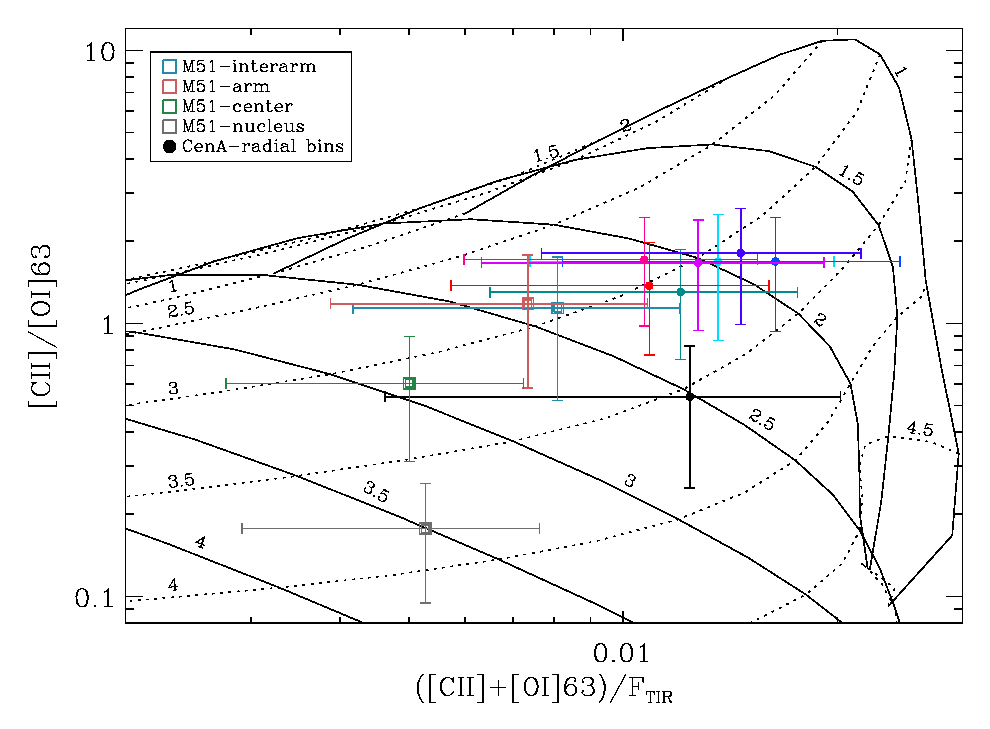
\includegraphics[width=\columnwidth]{CenA_CIIOI63_vs_CIIOI63onFtir_corrected_plot_radial_bins_wM51overlay_v2}
\caption{A comparison of the PDR model results for the radial bins of Cen~A with the PDR model results for the four regions in the inner region of M51 from \citet{parkin_2013}.}
\label{fig:pdr_comparison}
\end{figure}

The [O~\textsc{iii}]/[N~\textsc{ii}]$_{122}$ line ratio indicates that the youngest stars in Cen~A are hotter (O9.5 or O9) than in M51 \citep[B0; ][]{parkin_2013} based on the stellar classifications from \citet{1996ApJ...460..914V}.  This apparent discrepancy may be due to lower signal-to-noise in the M51 observations of the [O~\textsc{iii}] line than in Cen~A, which would indicate that the observed [O~\textsc{iii}]/[N~\textsc{ii}]$_122$ ratio in M51 from \citet{parkin_2013} is a lower limit, bringing the ratio closer to that observed in Cen~A.  It is also possible that the observed ratio is a combined effect of stars and the stronger AGN in Cen~A, thus making the apparent stellar classification earlier than it really is.

It appears that the physical characteristics of the PDRs in the molecular clouds of Cen~A are reasonably similar to those found in normal, star forming galaxies, although there seem to be a few noticeable differences between it and M51 based on our two data sets.

%%%%%%%%%%%%%%%%%%%%%%%%%%%%%%%%%%%%%%%%%
\section{Conclusions}\label{conclusions}
We have presented new spectroscopic observations of the unusual elliptical galaxy Centaurus~A from the \emph{Herschel} PACS instrument.  These observations focus on important atomic cooling lines originating from both neutral ([C~\textsc{ii}](158~$\mu$m), [O~\textsc{i}](63 and 145~$\mu$m)) and ionized gas ([N~\textsc{ii}](122 and 205~$\mu$m) and [O~\textsc{iii}](88~$\mu$m)) covering a radial strip on the eastern side of the nucleus of the galaxy (or a central aperture for the 205~$\mu$m line).  We divide our observational strip into eight bins radially to search for variations in the heating and cooling properties of the gas, as well as the characteristics of the PDR regions in the disk.

We find that the heating efficiency in the disk, represented by the ([C~\textsc{ii}]+[O~\textsc{i}]$_{63}$)/$F_{\mathrm{TIR}}$ line ratio, shows a slight increase with increasing radius from $4 \times 10^{-3}$ to $8 \times 10^{-3}$, consistent with values determined in galaxies on global scales, as well as on resolved scales in other individual galaxies.  Furthermore, the slightly suppressed heating efficiency suggests a harder radiation field in the region, likely from the AGN at the center.

A comparison beween a PDR model and our observations reveals that the strength of the FUV radiation field incident on the PDR surfaces ranges from $\sim 10^{1.75}$--10$^{2.75}$ and the hydrogen gas density ranges from $\sim 10^{2.75}$--$10^{3.75}$~cm$^{-3}$, in agreement with typical values in other star forming galaxies, as well as M82, which has a central starburst, and different from the elliptical galaxy NGC~4125.  However, we do not see a significant radial trend in either $n$ or $G_{0}$, in constrast to M51.  Furthermore, while the results from the PDR modelling for Cen~A agree with those for the arm and interarm regions in M51, the central region of M51 shows higher values for $n$ and $G_{0}$.  Observations of the nucleus of Cen~A in the important fine structure lines may reveal a similar trend; however, we point out that in the central region of M51 up to 70\% of the [C~\textsc{ii}] emission originates in diffuse ionized gas while in Cen~A this fraction is only 10--20\%, thus this may also explain the differences between the two galaxies.

We conclude that the disk of Cen~A exhibits properties in its molecular clouds that are similar to other normal disk galaxies, despite its unusual morphological characteristics.





%% If you wish to include an acknowledgments section in your paper,
%% separate it off from the body of the text using the \acknowledgments
%% command.

%% Included in this acknowledgments section are examples of the
%% AASTeX hypertext markup commands. Use \url without the optional [HREF]
%% argument when you want to print the url directly in the text. Otherwise,
%% use either \url or \anchor, with the HREF as the first argument and the
%% text to be printed in the second.

\acknowledgments
The research of C.~D.~W. is supported by the Natural Sciences and Engineering Research Council of Canada and the Canadian Space Agency.  PACS has been developed by a consortium of institutes led by MPE (Germany) and including UVIE (Austria); KU Leuven, CSL, IMEC (Belgium); CEA, LAM (France); MPIA (Germany); INAF-IFSI/OAA/OAP/OAT, LENS, SISSA (Italy); IAC (Spain). This development has been supported by the funding agencies BMVIT (Austria), ESA-PRODEX (Belgium), CEA/CNES (France), DLR (Germany), ASI/INAF (Italy), and CICYT/MCYT (Spain).  SPIRE has been developed by a consortium of institutes led by Cardiff University (UK) and including Univ. Lethbridge (Canada); NAOC (China); CEA, LAM (France); IFSI, Univ. Padua (Italy); IAC (Spain); Stockholm Observatory (Sweden); Imperial College London, RAL, UCL-MSSL, UKATC, Univ. Sussex (UK); and Caltech, JPL, NHSC, Univ. Colorado (USA). This development has been supported by national funding agencies: CSA (Canada); NAOC (China); CEA, CNES, CNRS (France); ASI (Italy); MCINN (Spain); SNSB (Sweden); STFC and UKSA (UK); and NASA (USA).  HIPE is a joint development by the Herschel Science Ground Segment Consortium, consisting of ESA, the NASA Herschel Science Center, and the HIFI, PACS and SPIRE consortia.  The James Clerk Maxwell Telescope is operated by The Joint Astronomy Centre on behalf of the Science and Technology Facilities Council of the United Kingdom, the Netherlands Organisation for Scientific Research, and the National Research Council of Canada. This research has made use of the NASA/IPAC Extragalactic Database (NED) which is operated by the Jet Propulsion Laboratory, California Institute of Technology, under contract with the National Aeronautics and Space Administration.  This research made use of APLpy, an open-source plotting package for Python hosted at http://aplpy.github.com.

%% To help institutions obtain information on the effectiveness of their
%% telescopes, the AAS Journals has created a group of keywords for telescope
%% facilities. A common set of keywords will make these types of searches
%% significantly easier and more accurate. In addition, they will also be
%% useful in linking papers together which utilize the same telescopes
%% within the framework of the National Virtual Observatory.
%% See the AASTeX Web site at http://www.journals.uchicago.edu/AAS/AASTeX
%% for information on obtaining the facility keywords.

%% After the acknowledgments section, use the following syntax and the
%% \facility{} macro to list the keywords of facilities used in the research
%% for the paper.  Each keyword will be checked against the master list during
%% copy editing.  Individual instruments or configurations can be provided 
%% in parentheses, after the keyword, but they will not be verified.

{\it Facilities:} \facility{Herschel (PACS, SPIRE)}.

%% Appendix material should be preceded with a single \appendix command.
%% There should be a \section command for each appendix. Mark appendix
%% subsections with the same markup you use in the main body of the paper.

%% Each Appendix (indicated with \section) will be lettered A, B, C, etc.
%% The equation counter will reset when it encounters the \appendix
%% command and will number appendix equations (A1), (A2), etc.

%% The reference list follows the main body and any appendices.
%% Use LaTeX's thebibliography environment to mark up your reference list.
%% Note \begin{thebibliography} is followed by an empty set of
%% curly braces.  If you forget this, LaTeX will generate the error
%% "Perhaps a missing \item?".
%%
%% thebibliography produces citations in the text using \bibitem-\cite
%% cross-referencing. Each reference is preceded by a
%% \bibitem command that defines in curly braces the KEY that corresponds
%% to the KEY in the \cite commands (see the first section above).
%% Make sure that you provide a unique KEY for every \bibitem or else the
%% paper will not LaTeX. The square brackets should contain
%% the citation text that LaTeX will insert in
%% place of the \cite commands.

%% We have used macros to produce journal name abbreviations.
%% AASTeX provides a number of these for the more frequently-cited journals.
%% See the Author Guide for a list of them.

%% Note that the style of the \bibitem labels (in []) is slightly
%% different from previous examples.  The natbib system solves a host
%% of citation expression problems, but it is necessary to clearly
%% delimit the year from the author name used in the citation.
%% See the natbib documentation for more details and options.

%% Commands to initiate bibliography:
%\bibliographystyle{apj}
%\bibliography{cena_bib}

\begin{thebibliography}{82}
\expandafter\ifx\csname natexlab\endcsname\relax\def\natexlab#1{#1}\fi

\bibitem[{{Abel} {et~al.}(2009){Abel}, {Dudley}, {Fischer}, {Satyapal}, \& {van
  Hoof}}]{2009ApJ...701.1147A}
{Abel}, N.~P., {Dudley}, C., {Fischer}, J., {Satyapal}, S., \& {van Hoof},
  P.~A.~M. 2009, \apj, 701, 1147

\bibitem[{{Aniano} {et~al.}(2011){Aniano}, {Draine}, {Gordon}, \&
  {Sandstrom}}]{2011PASP..123.1218A}
{Aniano}, G., {Draine}, B.~T., {Gordon}, K.~D., \& {Sandstrom}, K. 2011, \pasp,
  123, 1218

\bibitem[{{Bendo} {et~al.}(2012){Bendo}, {Galliano}, \&
  {Madden}}]{2012MNRAS.423..197B}
{Bendo}, G.~J., {Galliano}, F., \& {Madden}, S.~C. 2012, \mnras, 423, 197

\bibitem[{{Blum} \& {Pradhan}(1992)}]{1992ApJS...80..425B}
{Blum}, R.~D., \& {Pradhan}, A.~K. 1992, \apjs, 80, 425

\bibitem[{{Braine} {et~al.}(2012){Braine}, {Gratier}, {Kramer}, {Israel}, {van
  der Tak}, {Mookerjea}, {Boquien}, {Tabatabaei}, {van der Werf}, \&
  {Henkel}}]{2012A&A...544A..55B}
{Braine}, J., {Gratier}, P., {Kramer}, C., {et~al.} 2012, \aap, 544, A55

\bibitem[{{Brauher} {et~al.}(2008){Brauher}, {Dale}, \&
  {Helou}}]{2008ApJS..178..280B}
{Brauher}, J.~R., {Dale}, D.~A., \& {Helou}, G. 2008, \apjs, 178, 280

\bibitem[{{Calzetti} {et~al.}(2007){Calzetti}, {Kennicutt}, {Engelbracht},
  {Leitherer}, {Draine}, {Kewley}, {Moustakas}, {Sosey}, {Dale}, {Gordon},
  {Helou}, {Hollenbach}, {Armus}, {Bendo}, {Bot}, {Buckalew}, {Jarrett}, {Li},
  {Meyer}, {Murphy}, {Prescott}, {Regan}, {Rieke}, {Roussel}, {Sheth}, {Smith},
  {Thornley}, \& {Walter}}]{2007ApJ...666..870C}
{Calzetti}, D., {Kennicutt}, R.~C., {Engelbracht}, C.~W., {et~al.} 2007, \apj,
  666, 870

\bibitem[{{Calzetti} {et~al.}(2010){Calzetti}, {Wu}, {Hong}, {Kennicutt},
  {Lee}, {Dale}, {Engelbracht}, {van Zee}, {Draine}, {Hao}, {Gordon},
  {Moustakas}, {Murphy}, {Regan}, {Begum}, {Block}, {Dalcanton}, {Funes}, {Gil
  de Paz}, {Johnson}, {Sakai}, {Skillman}, {Walter}, {Weisz}, {Williams}, \&
  {Wu}}]{2010ApJ...714.1256C}
{Calzetti}, D., {Wu}, S.-Y., {Hong}, S., {et~al.} 2010, \apj, 714, 1256

\bibitem[{{Combi} \& {Romero}(1997)}]{1997A&AS..121...11C}
{Combi}, J.~A., \& {Romero}, G.~E. 1997, \aaps, 121, 11

\bibitem[{{Contursi} {et~al.}(2002){Contursi}, {Kaufman}, {Helou},
  {Hollenbach}, {Brauher}, {Stacey}, {Dale}, {Malhotra}, {Rubio}, {Rubin}, \&
  {Lord}}]{2002AJ....124..751C}
{Contursi}, A., {Kaufman}, M.~J., {Helou}, G., {et~al.} 2002, \aj, 124, 751

\bibitem[{{Contursi} {et~al.}(2013){Contursi}, {Poglitsch}, {Gr{\'a}cia
  Carpio}, {Veilleux}, {Sturm}, {Fischer}, {Verma}, {Hailey-Dunsheath}, {Lutz},
  {Davies}, {Gonz{\'a}lez-Alfonso}, {Sternberg}, {Genzel}, \&
  {Tacconi}}]{2013A&A...549A.118C}
{Contursi}, A., {Poglitsch}, A., {Gr{\'a}cia Carpio}, J., {et~al.} 2013, \aap,
  549, A118

\bibitem[{{Crawford} {et~al.}(1985){Crawford}, {Genzel}, {Townes}, \&
  {Watson}}]{1985ApJ...291..755C}
{Crawford}, M.~K., {Genzel}, R., {Townes}, C.~H., \& {Watson}, D.~M. 1985,
  \apj, 291, 755

\bibitem[{{Crocker} {et~al.}(2012){Crocker}, {Krips}, {Bureau}, {Young},
  {Davis}, {Bayet}, {Alatalo}, {Blitz}, {Bois}, {Bournaud}, {Cappellari},
  {Davies}, {de Zeeuw}, {Duc}, {Emsellem}, {Khochfar}, {Krajnovi{\'c}},
  {Kuntschner}, {Lablanche}, {McDermid}, {Morganti}, {Naab}, {Oosterloo},
  {Sarzi}, {Scott}, {Serra}, \& {Weijmans}}]{2012MNRAS.421.1298C}
{Crocker}, A., {Krips}, M., {Bureau}, M., {et~al.} 2012, \mnras, 421, 1298

\bibitem[{{Crocker} {et~al.}(2011){Crocker}, {Bureau}, {Young}, \&
  {Combes}}]{2011MNRAS.410.1197C}
{Crocker}, A.~F., {Bureau}, M., {Young}, L.~M., \& {Combes}, F. 2011, \mnras,
  410, 1197

\bibitem[{{Croxall} {et~al.}(2012){Croxall}, {Smith}, {Wolfire}, {Roussel},
  {Sandstrom}, {Draine}, {Aniano}, {Dale}, {Armus}, {Beir{\~a}o}, {Helou},
  {Bolatto}, {Appleton}, {Brandl}, {Calzetti}, {Crocker}, {Galametz}, {Groves},
  {Hao}, {Hunt}, {Johnson}, {Kennicutt}, {Koda}, {Krause}, {Li}, {Meidt},
  {Murphy}, {Rahman}, {Rix}, {Sauvage}, {Schinnerer}, {Walter}, \&
  {Wilson}}]{2012ApJ...747...81C}
{Croxall}, K.~V., {Smith}, J.~D., {Wolfire}, M.~G., {et~al.} 2012, \apj, 747,
  81

\bibitem[{{Eckart} {et~al.}(1990){Eckart}, {Cameron}, {Rothermel}, {Wild},
  {Zinnecker}, {Rydbeck}, {Olberg}, \& {Wiklind}}]{1990ApJ...363..451E}
{Eckart}, A., {Cameron}, M., {Rothermel}, H., {et~al.} 1990, \apj, 363, 451

\bibitem[{{Ferkinhoff} {et~al.}(2011){Ferkinhoff}, {Brisbin}, {Nikola},
  {Parshley}, {Stacey}, {Phillips}, {Falgarone}, {Benford}, {Staguhn}, \&
  {Tucker}}]{2011ApJ...740L..29F}
{Ferkinhoff}, C., {Brisbin}, D., {Nikola}, T., {et~al.} 2011, \apjl, 740, L29

\bibitem[{{Galametz} {et~al.}(2013){Galametz}, {Kennicutt}, {Calzetti},
  {Aniano}, {Draine}, {Boquien}, {Brandl}, {Croxall}, {Dale}, {Engelbracht},
  {Gordon}, {Groves}, {Hao}, {Helou}, {Hinz}, {Hunt}, {Johnson}, {Li},
  {Murphy}, {Roussel}, {Sandstrom}, {Skibba}, \&
  {Tabatabaei}}]{2013MNRAS.431.1956G}
{Galametz}, M., {Kennicutt}, R.~C., {Calzetti}, D., {et~al.} 2013, \mnras, 431,
  1956

\bibitem[{{Galavis} {et~al.}(1997){Galavis}, {Mendoza}, \&
  {Zeippen}}]{1997A&AS..123..159G}
{Galavis}, M.~E., {Mendoza}, C., \& {Zeippen}, C.~J. 1997, \aaps, 123, 159

\bibitem[{{Galavis} {et~al.}(1998){Galavis}, {Mendoza}, \&
  {Zeippen}}]{1998A&AS..131..499G}
---. 1998, \aaps, 131, 499

\bibitem[{{Graci{\'a}-Carpio} {et~al.}(2008){Graci{\'a}-Carpio},
  {Garc{\'{\i}}a-Burillo}, {Planesas}, {Fuente}, \&
  {Usero}}]{2008A&A...479..703G}
{Graci{\'a}-Carpio}, J., {Garc{\'{\i}}a-Burillo}, S., {Planesas}, P., {Fuente},
  A., \& {Usero}, A. 2008, \aap, 479, 703

\bibitem[{{Graci{\'a}-Carpio} {et~al.}(2011){Graci{\'a}-Carpio}, {Sturm},
  {Hailey-Dunsheath}, {Fischer}, {Contursi}, {Poglitsch}, {Genzel},
  {Gonz{\'a}lez-Alfonso}, {Sternberg}, {Verma}, {Christopher}, {Davies},
  {Feuchtgruber}, {de Jong}, {Lutz}, \& {Tacconi}}]{2011ApJ...728L...7G}
{Graci{\'a}-Carpio}, J., {Sturm}, E., {Hailey-Dunsheath}, S., {et~al.} 2011,
  \apjl, 728, L7

\bibitem[{{Griffin} {et~al.}(2010)}]{2010A&A...518L...3G}
{Griffin}, M.~J., {et~al.} 2010, \aap, 518, L3

\bibitem[{{Groves} {et~al.}(2004){Groves}, {Dopita}, \&
  {Sutherland}}]{2004ApJS..153....9G}
{Groves}, B.~A., {Dopita}, M.~A., \& {Sutherland}, R.~S. 2004, \apjs, 153, 9

\bibitem[{{Habing}(1968)}]{1968BAN....19..421H}
{Habing}, H.~J. 1968, \bain, 19, 421

\bibitem[{{Harris} {et~al.}(2010){Harris}, {Rejkuba}, \&
  {Harris}}]{2010PASA...27..457H}
{Harris}, G.~L.~H., {Rejkuba}, M., \& {Harris}, W.~E. 2010, \pasa, 27, 457

\bibitem[{{Ho} {et~al.}(1997){Ho}, {Filippenko}, \&
  {Sargent}}]{1997ApJS..112..315H}
{Ho}, L.~C., {Filippenko}, A.~V., \& {Sargent}, W.~L.~W. 1997, \apjs, 112, 315

\bibitem[{{Hollenbach} \& {McKee}(1989)}]{1989ApJ...342..306H}
{Hollenbach}, D., \& {McKee}, C.~F. 1989, \apj, 342, 306

\bibitem[{{Hollenbach} {et~al.}(1991){Hollenbach}, {Takahashi}, \&
  {Tielens}}]{1991ApJ...377..192H}
{Hollenbach}, D.~J., {Takahashi}, T., \& {Tielens}, A.~G.~G.~M. 1991, \apj,
  377, 192

\bibitem[{{Hudson} \& {Bell}(2004)}]{2004MNRAS.348.1275H}
{Hudson}, C.~E., \& {Bell}, K.~L. 2004, \mnras, 348, 1275

\bibitem[{{Israel}(1998)}]{1998A&ARv...8..237I}
{Israel}, F.~P. 1998, \aapr, 8, 237

\bibitem[{{Kaufman} {et~al.}(2006){Kaufman}, {Wolfire}, \&
  {Hollenbach}}]{2006ApJ...644..283K}
{Kaufman}, M.~J., {Wolfire}, M.~G., \& {Hollenbach}, D.~J. 2006, \apj, 644, 283

\bibitem[{{Kaufman} {et~al.}(1999){Kaufman}, {Wolfire}, {Hollenbach}, \&
  {Luhman}}]{1999ApJ...527..795K}
{Kaufman}, M.~J., {Wolfire}, M.~G., {Hollenbach}, D.~J., \& {Luhman}, M.~L.
  1999, \apj, 527, 795

\bibitem[{{Kennicutt}(1998)}]{1998ApJ...498..541K}
{Kennicutt}, Jr., R.~C. 1998, \apj, 498, 541

\bibitem[{{Kennicutt} {et~al.}(2007){Kennicutt}, {Calzetti}, {Walter}, {Helou},
  {Hollenbach}, {Armus}, {Bendo}, {Dale}, {Draine}, {Engelbracht}, {Gordon},
  {Prescott}, {Regan}, {Thornley}, {Bot}, {Brinks}, {de Blok}, {de Mello},
  {Meyer}, {Moustakas}, {Murphy}, {Sheth}, \& {Smith}}]{2007ApJ...671..333K}
{Kennicutt}, Jr., R.~C., {Calzetti}, D., {Walter}, F., {et~al.} 2007, \apj,
  671, 333

\bibitem[{{Kennicutt} {et~al.}(2009){Kennicutt}, {Hao}, {Calzetti},
  {Moustakas}, {Dale}, {Bendo}, {Engelbracht}, {Johnson}, \&
  {Lee}}]{2009ApJ...703.1672K}
{Kennicutt}, Jr., R.~C., {Hao}, C.-N., {Calzetti}, D., {et~al.} 2009, \apj,
  703, 1672

\bibitem[{{Kramer} {et~al.}(2005){Kramer}, {Mookerjea}, {Bayet},
  {Garcia-Burillo}, {Gerin}, {Israel}, {Stutzki}, \&
  {Wouterloot}}]{2005A&A...441..961K}
{Kramer}, C., {Mookerjea}, B., {Bayet}, E., {et~al.} 2005, \aap, 441, 961

\bibitem[{{Le Petit} {et~al.}(2006){Le Petit}, {Nehm{\'e}}, {Le Bourlot}, \&
  {Roueff}}]{2006ApJS..164..506L}
{Le Petit}, F., {Nehm{\'e}}, C., {Le Bourlot}, J., \& {Roueff}, E. 2006, \apjs,
  164, 506

\bibitem[{{Lebouteiller} {et~al.}(2012){Lebouteiller}, {Cormier}, {Madden},
  {Galliano}, {Indebetouw}, {Abel}, {Sauvage}, {Hony}, {Contursi}, {Poglitsch},
  {R{\'e}my}, {Sturm}, \& {Wu}}]{2012A&A...548A..91L}
{Lebouteiller}, V., {Cormier}, D., {Madden}, S.~C., {et~al.} 2012, \aap, 548,
  A91

\bibitem[{{Leeuw} {et~al.}(2002){Leeuw}, {Hawarden}, {Matthews}, {Robson}, \&
  {Eckart}}]{2002ApJ...565..131L}
{Leeuw}, L.~L., {Hawarden}, T.~G., {Matthews}, H.~E., {Robson}, E.~I., \&
  {Eckart}, A. 2002, \apj, 565, 131

\bibitem[{{Li} {et~al.}(2013){Li}, {Crocker}, {Calzetti}, {Wilson},
  {Kennicutt}, {Murphy}, {Brandl}, {Draine}, {Galametz}, {Johnson}, {Armus},
  {Gordon}, {Croxall}, {Dale}, {Engelbracht}, {Groves}, {Hao}, {Helou}, {Hinz},
  {Hunt}, {Krause}, {Roussel}, {Sauvage}, \& {Smith}}]{2013ApJ...768..180L}
{Li}, Y., {Crocker}, A.~F., {Calzetti}, D., {et~al.} 2013, \apj, 768, 180

\bibitem[{{Luhman} {et~al.}(1997){Luhman}, {Jaffe}, {Sternberg}, {Herrmann}, \&
  {Poglitsch}}]{1997ApJ...482..298L}
{Luhman}, M.~L., {Jaffe}, D.~T., {Sternberg}, A., {Herrmann}, F., \&
  {Poglitsch}, A. 1997, \apj, 482, 298

\bibitem[{{Luhman} {et~al.}(2003){Luhman}, {Satyapal}, {Fischer}, {Wolfire},
  {Sturm}, {Dudley}, {Lutz}, \& {Genzel}}]{2003ApJ...594..758L}
{Luhman}, M.~L., {Satyapal}, S., {Fischer}, J., {et~al.} 2003, \apj, 594, 758

\bibitem[{{Luhman} {et~al.}(1998){Luhman}, {Satyapal}, {Fischer}, {Wolfire},
  {Cox}, {Lord}, {Smith}, {Stacey}, \& {Unger}}]{1998ApJ...504L..11L}
---. 1998, \apjl, 504, L11

\bibitem[{{Malhotra} {et~al.}(2001){Malhotra}, {Kaufman}, {Hollenbach},
  {Helou}, {Rubin}, {Brauher}, {Dale}, {Lu}, {Lord}, {Stacey}, {Contursi},
  {Hunter}, \& {Dinerstein}}]{2001ApJ...561..766M}
{Malhotra}, S., {Kaufman}, M.~J., {Hollenbach}, D., {et~al.} 2001, \apj, 561,
  766

\bibitem[{{Mookerjea} {et~al.}(2011){Mookerjea}, {Kramer}, {Buchbender},
  {Boquien}, {Verley}, {Rela{\~n}o}, {Quintana-Lacaci}, {Aalto}, {Braine},
  {Calzetti}, {Combes}, {Garcia-Burillo}, {Gratier}, {Henkel}, {Israel},
  {Lord}, {Nikola}, {R{\"o}llig}, {Stacey}, {Tabatabaei}, {van der Tak}, \&
  {van der Werf}}]{2011A&A...532A.152M}
{Mookerjea}, B., {Kramer}, C., {Buchbender}, C., {et~al.} 2011, \aap, 532, A152

\bibitem[{{Morganti}(2010)}]{2010PASA...27..463M}
{Morganti}, R. 2010, \pasa, 27, 463

\bibitem[{{Morganti} {et~al.}(2008){Morganti}, {Oosterloo}, {Struve}, \&
  {Saripalli}}]{2008A&A...485L...5M}
{Morganti}, R., {Oosterloo}, T., {Struve}, C., \& {Saripalli}, L. 2008, \aap,
  485, L5

\bibitem[{{Negishi} {et~al.}(2001){Negishi}, {Onaka}, {Chan}, \&
  {Roellig}}]{2001A&A...375..566N}
{Negishi}, T., {Onaka}, T., {Chan}, K.-W., \& {Roellig}, T.~L. 2001, \aap, 375,
  566

\bibitem[{{Oberst} {et~al.}(2006){Oberst}, {Parshley}, {Stacey}, {Nikola},
  {L{\"o}hr}, {Harnett}, {Tothill}, {Lane}, {Stark}, \&
  {Tucker}}]{2006ApJ...652L.125O}
{Oberst}, T.~E., {Parshley}, S.~C., {Stacey}, G.~J., {et~al.} 2006, \apjl, 652,
  L125

\bibitem[{{Ott}(2010)}]{2010ASPC..434..139O}
{Ott}, S. 2010, in Astronomical Society of the Pacific Conference Series, Vol.
  434, Astronomical Data Analysis Software and Systems XIX, ed. {Y.~Mizumoto,
  K.-I.~Morita, \& M.~Ohishi}, 139--+

\bibitem[{{Parkin} {et~al.}(2012){Parkin}, {Wilson}, {Foyle}, {Baes}, {Bendo},
  {Boselli}, {Boquien}, {Cooray}, {Cormier}, {Davies}, {Eales}, {Galametz},
  {Gomez}, {Lebouteiller}, {Madden}, {Mentuch}, {Page}, {Pohlen}, {Remy},
  {Roussel}, {Sauvage}, {Smith}, \& {Spinoglio}}]{2012MNRAS.422.2291P}
{Parkin}, T.~J., {Wilson}, C.~D., {Foyle}, K., {et~al.} 2012, \mnras, 422, 2291

\bibitem[{{Parkin} {et~al.}(2013)}]{parkin_2013}
{Parkin}, T.~J., {et~al.} 2013, submitted to \apj

\bibitem[{{Phillips} {et~al.}(1987){Phillips}, {Ellison}, {Keene}, {Leighton},
  {Howard}, {Masson}, {Sanders}, {Veidt}, \& {Young}}]{1987ApJ...322L..73P}
{Phillips}, T.~G., {Ellison}, B.~N., {Keene}, J.~B., {et~al.} 1987, \apjl, 322,
  L73

\bibitem[{{Pilbratt} {et~al.}(2010)}]{2010A&A...518L...1P}
{Pilbratt}, G.~L., {et~al.} 2010, \aap, 518, L1

\bibitem[{{Poglitsch} {et~al.}(2010)}]{2010A&A...518L...2P}
{Poglitsch}, A., {et~al.} 2010, \aap, 518, L2

\bibitem[{{Quillen} {et~al.}(2006){Quillen}, {Brookes}, {Keene}, {Stern},
  {Lawrence}, \& {Werner}}]{2006ApJ...645.1092Q}
{Quillen}, A.~C., {Brookes}, M.~H., {Keene}, J., {et~al.} 2006, \apj, 645, 1092

\bibitem[{{Quillen} {et~al.}(1992){Quillen}, {de Zeeuw}, {Phinney}, \&
  {Phillips}}]{1992ApJ...391..121Q}
{Quillen}, A.~C., {de Zeeuw}, P.~T., {Phinney}, E.~S., \& {Phillips}, T.~G.
  1992, \apj, 391, 121

\bibitem[{{R{\"o}llig} {et~al.}(2006){R{\"o}llig}, {Ossenkopf}, {Jeyakumar},
  {Stutzki}, \& {Sternberg}}]{2006A&A...451..917R}
{R{\"o}llig}, M., {Ossenkopf}, V., {Jeyakumar}, S., {Stutzki}, J., \&
  {Sternberg}, A. 2006, \aap, 451, 917

\bibitem[{{Rubin}(1985)}]{1985ApJS...57..349R}
{Rubin}, R.~H. 1985, \apjs, 57, 349

\bibitem[{{Rydbeck} {et~al.}(1993){Rydbeck}, {Wiklind}, {Cameron}, {Wild},
  {Eckart}, {Genzel}, \& {Rothermel}}]{1993A&A...270L..13R}
{Rydbeck}, G., {Wiklind}, T., {Cameron}, M., {et~al.} 1993, \aap, 270, L13

\bibitem[{{Savage} \& {Sembach}(1996)}]{1996ARA&A..34..279S}
{Savage}, B.~D., \& {Sembach}, K.~R. 1996, \araa, 34, 279

\bibitem[{{Stacey} {et~al.}(1991){Stacey}, {Geis}, {Genzel}, {Lugten},
  {Poglitsch}, {Sternberg}, \& {Townes}}]{1991ApJ...373..423S}
{Stacey}, G.~J., {Geis}, N., {Genzel}, R., {et~al.} 1991, \apj, 373, 423

\bibitem[{{Stacey} {et~al.}(1993){Stacey}, {Jaffe}, {Geis}, {Grenzel},
  {Harris}, {Poglitsch}, {Stutzki}, \& {Townes}}]{1993ApJ...404..219S}
{Stacey}, G.~J., {Jaffe}, D.~T., {Geis}, N., {et~al.} 1993, \apj, 404, 219

\bibitem[{{Stacey} {et~al.}(1985){Stacey}, {Viscuso}, {Fuller}, \&
  {Kurtz}}]{1985ApJ...289..803S}
{Stacey}, G.~J., {Viscuso}, P.~J., {Fuller}, C.~E., \& {Kurtz}, N.~T. 1985,
  \apj, 289, 803

\bibitem[{{Sternberg} \& {Dalgarno}(1989)}]{1989ApJ...338..197S}
{Sternberg}, A., \& {Dalgarno}, A. 1989, \apj, 338, 197

\bibitem[{{Sternberg} \& {Dalgarno}(1995)}]{1995ApJS...99..565S}
---. 1995, \apjs, 99, 565

\bibitem[{{St{\"o}rzer} {et~al.}(2000){St{\"o}rzer}, {Zielinsky}, {Stutzki}, \&
  {Sternberg}}]{2000A&A...358..682S}
{St{\"o}rzer}, H., {Zielinsky}, M., {Stutzki}, J., \& {Sternberg}, A. 2000,
  \aap, 358, 682

\bibitem[{{Strong} {et~al.}(1988){Strong}, {Bloemen}, {Dame}, {Grenier},
  {Hermsen}, {Lebrun}, {Nyman}, {Pollock}, \& {Thaddeus}}]{1988A&A...207....1S}
{Strong}, A.~W., {Bloemen}, J.~B.~G.~M., {Dame}, T.~M., {et~al.} 1988, \aap,
  207, 1

\bibitem[{{Struve} {et~al.}(2010){Struve}, {Oosterloo}, {Morganti}, \&
  {Saripalli}}]{2010A&A...515A..67S}
{Struve}, C., {Oosterloo}, T.~A., {Morganti}, R., \& {Saripalli}, L. 2010,
  \aap, 515, A67+

\bibitem[{{Tielens} \& {Hollenbach}(1985)}]{1985ApJ...291..722T}
{Tielens}, A.~G.~G.~M., \& {Hollenbach}, D. 1985, \apj, 291, 722

\bibitem[{{Tubbs}(1980)}]{1980ApJ...241..969T}
{Tubbs}, A.~D. 1980, \apj, 241, 969

\bibitem[{{Unger} {et~al.}(2000){Unger}, {Clegg}, {Stacey}, {Cox}, {Fischer},
  {Greenhouse}, {Lord}, {Luhman}, {Satyapal}, {Smith}, {Spinoglio}, \&
  {Wolfire}}]{2000A&A...355..885U}
{Unger}, S.~J., {Clegg}, P.~E., {Stacey}, G.~J., {et~al.} 2000, \aap, 355, 885

\bibitem[{{Vacca} {et~al.}(1996){Vacca}, {Garmany}, \&
  {Shull}}]{1996ApJ...460..914V}
{Vacca}, W.~D., {Garmany}, C.~D., \& {Shull}, J.~M. 1996, \apj, 460, 914

\bibitem[{{van Dishoeck} \& {Black}(1986)}]{1986ApJS...62..109V}
{van Dishoeck}, E.~F., \& {Black}, J.~H. 1986, \apjs, 62, 109

\bibitem[{{van Dishoeck} \& {Black}(1988)}]{1988ApJ...334..771V}
---. 1988, \apj, 334, 771

\bibitem[{{Wei{\ss}} {et~al.}(2008){Wei{\ss}}, {Kov{\'a}cs}, {G{\"u}sten},
  {Menten}, {Schuller}, {Siringo}, \& {Kreysa}}]{2008A&A...490...77W}
{Wei{\ss}}, A., {Kov{\'a}cs}, A., {G{\"u}sten}, R., {et~al.} 2008, \aap, 490,
  77

\bibitem[{{Welch} {et~al.}(2010){Welch}, {Sage}, \&
  {Young}}]{2010ApJ...725..100W}
{Welch}, G.~A., {Sage}, L.~J., \& {Young}, L.~M. 2010, \apj, 725, 100

\bibitem[{{Wilson} {et~al.}(2009)}]{2009ApJ...693.1736W}
{Wilson}, C.~D., {et~al.} 2009, \apj, 693, 1736

\bibitem[{{Wolfire} {et~al.}(1990){Wolfire}, {Tielens}, \&
  {Hollenbach}}]{1990ApJ...358..116W}
{Wolfire}, M.~G., {Tielens}, A.~G.~G.~M., \& {Hollenbach}, D. 1990, \apj, 358,
  116

\bibitem[{{Wu} {et~al.}(2005){Wu}, {Cao}, {Hao}, {Liu}, {Wang}, {Xia}, {Deng},
  \& {Young}}]{2005ApJ...632L..79W}
{Wu}, H., {Cao}, C., {Hao}, C.-N., {et~al.} 2005, \apjl, 632, L79

\bibitem[{{Young} {et~al.}(2011)}]{2011MNRAS.414..940Y}
{Young}, L.~M., {et~al.} 2011, \mnras, 414, 940

\end{thebibliography}


\end{document}

%%
%% End of file `sample.tex'.
